%
% Tallinn University of Technology - bachelor, master thesis template for LaTeX
%
% Public Version 1.1
% 2019 Adjusted by Frank Korving for his Bachelor Thesis, with contributions from Sander Arnus
%
% Public version 1.0
% 2010 - 2013 Thijs Nugteren and Joos Buijs for Master Thesis
%
% THIS IS THE MAIN FILE (i.e. compile this file, compiling the others directly won't work)
%
\documentclass[12pt, a4paper]{report}

% all the other includes etc. are done in the thesis.sty file.
\usepackage{thesis}
\usepackage{biblatex}

%
% These commands need to be defined in order to produce a correct and personalized document
%
\newcommand{\doctitle}{Development of Time Tracking and Visualization System for Programming}
% Programmeerimisele kuluva aja jälgimise ja visualiseerimise süsteemi arendamine
\newcommand{\docsubtitle}{Bachelor Thesis}

\newcommand{\meone}{Tavo Annus}
\newcommand{\metwo}{Marten Jürgenson}
\newcommand{\studentcodeone}{186060IAIB}
\newcommand{\studentcodetwo}{185045IAIB}
\newcommand{\university}{TALLINN UNIVERSITY OF TECHNOLOGY}
\newcommand{\school}{School of Information Technologies}
\newcommand{\department}{Department of Software Science}

\newcommand{\supervisor}{Ago Luberg}
\newcommand{\supervisortitle}{M Sc}
\newcommand{\cosupervisor}{Secondary Supervisor Name}
\newcommand{\cosupervisortitle}{MsC}
\newcommand{\keywords}{gtm, time tracking, git, rust, go, react, jetbrains}
\newcommand{\version}{1.0 version}
\newcommand{\monthYear}{May 18th}
\newcommand{\Year}{2021}
\newcommand{\signatureDate}{May 18th, 2021}

\author{\meone \metwo}

%
% PDF settings
%
\hypersetup
{
    pdfauthor={\meone \metwo},
pdfsubject={\doctitle},
pdfkeywords={\keywords}
}

\begin{document}
    \pagenumbering{roman}
    \begin{titlepage}
    \headheight = 57pt
    \footskip = 5pt
    \headsep = 0pt

    \centering
    \textsc{\begin{Large}
                \university\\
    \end{Large} }
    \school\\
    \department\\

    \vspace*{7 cm}

    \begin{center}

        \meone \quad \studentcodeone\\
        \metwo \quad \studentcodetwo\\
        \begin{Large}
            \textsc{\textbf{\doctitle}}\\
        \end{Large}
        \docsubtitle\\
    \end{center}

    \begin{flushright}
        \textbf{Supervisor}\\ \supervisor\\\supervisortitle\\
        % \textbf{Academic Supervisor}\\\cosupervisor\\\cosupervisortitle
    \end{flushright}

    \vfill

    Tallinn \Year
\end{titlepage}

    \normalsize

    \chapter*{\centerline{Author's declaration of originality}}\label{chapter:declaration}
    \hfill \\
I hereby certify that I am the sole author of this thesis. All the used materials, references
to the literature and the work of others have been referred to. This thesis has not been
presented for examination anywhere else.

\vskip1in
\begin{flushleft}
    \begin{tabular}{p{2.0cm}p{6.0cm}p{4.0cm}}
        Author: & \meone, \metwo & ......................................\\
        && \hfill(signature)\\
        Date: & \signatureDate &\\
        \\
        \\

% Uncomment the following to add supervisor declaration
%  \multicolumn{3}{l}{The thesis adheres to all specified requirements}\\
%  \hfill \\
%  Supervisor: & \supervisor & ......................................\\
%  && \hfill(signature)\\
%  Date: & \signatureDate &\\


    \end{tabular}
\end{flushleft}

    \chapter*{\centerline{Annotatsioon}}\label{chapter:abstract-eesti}
    Lõputöö on kirjutatud ... keeles ning sisaldab teksti ... leheküljel, ... peatükki, ... joonist, ... tabelit.
    \pagebreak

    \chapter*{\centerline{Abstract}}\label{chapter:abstract}
    As part of this thesis, open source time tracking system was build for Tallinn University of Technology.
The purpose of the system is to give an overview of the time put into each task and how is
this effort is distributed over time.
The system is built for both lecturers and students, and it is developed in a way that it
could be also used for personal projects or companies.

The system is built around an open source app called \href{https://github.com/git-time-metric/gtm}{Git-Time-Metric}.
Now the system consists of five different applications distributed into five layers.
Two of the layers are on a client machine and three are hosted on a server.
Rust, Go, TypeScript and Kotlin programming languages were used in writing the applications.

As a result of this work, \href{https://github.com/git-time-metric/gtm}{Git-Time-Metric} app was improved,
a plugin was built for Jetbrains' editors,
a Debian package was built for the app responsible for collecting data from multiple Git repositories
and a frontend - backend combo was built for storing and visualizing data.

Deployed web app is accessible at \href{https://cs.ttu.ee/services/gtm/front}{https://cs.ttu.ee/services/gtm/front}
and rest of the applications can be found on GitHub \href{https://github.com/DEVELOPEST}{https://github.com/DEVELOPEST}.

The thesis is in English and contains 46 pages of text, 7 chapters, 19 figures, 14 tables.
    \pagebreak

    \chapter*{\centerline{List of abbreviations and terms}}\label{chapter:terms}
    \begin{longtable}{p{3cm}p{10cm}}
    API&Application Programming Interface\\
    BSD-3&Berkeley Software Distribution 3 Clause Licence\\
    CI/CD&Continuous Integration and Continuous Development\\
    CLI&Command Line Interface\\
    CSV&Comma Separated Values\\
    DDD&Domain Driven Design\\
    ERD&Entity Relationship Diagram\\
    GPLv3&GNU General Public License v3.0\\
    HTTP&Hyper Text Transfer Protocol\\
    IDE&Integrated Development Environment\\
    JSON&Java Script Object Notation\\
    JWT&JSON Web Token\\
    LGPLv3&GNU Lesser General Public License v3.0\\
    MIT&Massachusetts Institute of Technology\\
    ORM&Object-relational mapping\\
    REST&Representational State Transfer\\
    SQL&Structured Query Language\\
    SSH&Secure Shell Protocol\\
    VCS&Version Control System\\
\end{longtable}
\addtocounter{table}{-1}

    \pagebreak

    \phantomsection
    \setcounter{tocdepth}{2}    % Sets maximum depth of Table Of Contents
    \renewcommand{\contentsname}{Table of Contents}
    \tableofcontents

    \clearpage \phantomsection
    \setcounter{figure}{0}
    \addcontentsline{toc}{chapter}{\listfigurename}
    \listoffigures

    \clearpage \phantomsection
    \addcontentsline{toc}{chapter}{\listtablename}
    \listoftables

    \chapter{Introduction}\label{ch:introduction}
    \onehalfspacing
    \setcounter{page}{0}
    \pagenumbering{arabic}   %from here on, start the 'real' page numbering, from 1, with normal digits
    In programs development it is very important to have an estimate of how long developing different parts of application takes as
developer work hours make up big part of application cost.
This estimate can be calculated from time spent on writing similar tasks from past.

Similarly, it is important to have general idea of how much time students spend on different subjects in university.
All subjects have some time estimate but subjects with similar time estimate still tend to be very different in actual
time needed for completion.
Therefore, a solution is needed to track actual time spent on subjects.

In subjects mostly consisting of programming exercises this can be achieved by tracking time spent on writing and testing programs.
As it is very common to use Git for code management both at universities and companies linking time tracking to git commits
gives opportunity to also have statistics such as time spent per commit and lines written per commit.

To protect source code in non-public repositories it is important to have architecture in which parts accessing code are
installed into client server and are open source so that client can ensure there is no sensible data leaked.

Due to Git being command line tool also a separate graphical application is needed for visualizing data collected
from Git projects.

???

    \chapter{Project description}\label{ch:project-description}
    Prior to the actual development, the general project framework was sey up:
\begin{itemize}
    \item The roles and responsibilities were split.
    \item The rules and agreements on developing methodology were made.
    \item Environments were set up
\end{itemize}

It was agreed that Tavo Annus is responsible for DevOps and client side software.
Marten Jürgenson is responsible for a backend and frontend development.
As the client side software has less work to do, Tavo will be also working on both backend and
frontend on the later half of the project.

For the project management, GitHub was chosen as it is more common for users to browse project on GitHub rather than Gitlab.
Universities personal Gitlab server was ruled out as it does not allow non-university students to easily access open source parts of our application.

As a communication channel, Discord was used for both text and sound/video communication.
The main reason was that we were both used to using Discord, it is free, and it allows reasonably well formatted code pastes / pinning.

Meetings with TalTech mentor were organized weekly on Teams to have continuous feedback on project.

\section{Existing solutions}\label{sec:existing-solutions}
Before application design, some research was done to find already existing solutions.
The purpose of this task was to find out, if we could partially use some other programs and also get better understanding how
this kind of application could be built.


\subsection{Wakatime}\label{subsec:wakatime}
\href{https://wakatime.com/about}{Wakatime} is one of most popular applications used for tracking your work.
It supports variety of Integrated Development Environments (IDEs) including JetBrains IDEs required by TalTech.
It has both it's IDE plugins and Command Line Interface (CLI) app licenced under BSD-3 licence.
It also has a public API that allows fetching time data from their servers.
The downside of using Wakatime is that firstly it costs to see data older than 2 weeks and as it only temporarily
stores data on client machine, there is no easy way to access data without modifying already existent CLI app.
Wakatime also does not make use git statistics such as lines added and lines removed.
It only reads branch name, commit message and author data.
The reason behind this is likely it's architecture - it continuously sends heartbeats with required data to it's backed.
If no internet connection exists, it stores these heartbeats locally in rather cryptic format.
As a result there is not much data stored locally meaning that the backend has to bundle time data to commits which becomes a very complicated task
once users start rewriting history, especially given that Git is a distributed version control system.


\subsection{Git-Time-Metric}\label{subsec:git-time-metric}
\href{https://github.com/git-time-metric/gtm}{Git-Time-Metric} is a popular open source time tracking plugin licenced under MIT licence.
It has plugins for most commonly used IDEs including JetBrains IDEs, VSCode, Vim and more.
It is closely tied to git as it stores it's time tracking data in git notes.
This allows it to access more Git data such as lines added and lines removed for each commit.
Git-Time-Metric does not have a web interface (there are some half done projects meant to run only locally).
On the other hand, it has a very powerful and pretty CLI also capable of displaying data in a human-readable format.

One of the biggest downsides of Git-Time-Metric is that its active development has stopped in August 2019 and also it's plugins haven't received many updates.
Since JetBrains IDEs have changed a lot since that time it doesn't work on newest IDE versions making it tricky to use.

The biggest design difference between~\nameref{subsec:wakatime} and Git-Time-Metric is that Git-Time-Metric stores all it's data locally.
This makes the Git repository own it's time tracking data and not to worry about external companies policies.
There is always a CLI app capable of continuing to record and also display the data tracked.


\subsection{DarkyenusTimeTracker}\label{subsec:darkyenus-time-tracker}
\href{https://github.com/Darkyenus/DarkyenusTimeTracker}{DarkyenusTimeTracker} is also an open source time tracker licenced under The Unlicensed.
It is only a plugin built for JetBrains IDEs, but it does support automatic recording.
It only stores time since last commit, but it does support automatic time logging to commit messages meaning that this data can be possibly collected via Jira or some other software.
Sadly Gitlab, nor Github currently support parsing time data from git commit messages (Gitlab only support time logging directly under issue).
The other downside is that it only logs the total amount of time spent, no per file statistics.

Similarly to
\ref{subsec:git-time-metric}, it does not have a web interface, and it would be very hard to make one as the time date is not clearly separated from Git commit messages.
It also doesn't have a CLI interface due to similar reasons as web app.

\subsection{Existing plugin analysis results}\label{subsec:existing-plugin-analysis-results}
During the analysis there were two main ideas which way to go:
\begin{enumerate}
    \item Build a Git statistics support for~\nameref{subsec:wakatime}.
    \item Add some features to~\nameref{subsec:git-time-metric} and rebuild (some of) its plugins.
\end{enumerate}

\nameref{subsec:darkyenus-time-tracker} was ruled out as it lacked features useful for us.
Non the less, it was decided that we can use it as a base for building JetBrains plugin.

Building a Git statistics support for~\nameref{subsec:wakatime} also requires us to build our own backed for all the data or pay to access~\nameref{subsec:wakatime} API.
Either way an external database is needed to store all its Git related statistics.
Whilst it has great benefits, it is very hard to implement as it would require adding extra features to all most all it's plugins.
As Git history rewrites may cause conflicts it also needs either a complex system to solve these conflicts or just ignore history overwrites.
The second option would mean that whilst the time data saved would very closely reflect developer work in the short term it might get
confusing in the long run.
As a result of numerous rebases and squashes in different branches it becomes difficult to understand where the time data belongs.
The question arises: Why would we want to have time data attached to manny commits if don't really care about the commits and just squash them?
For us the answer was that we should also squash the time data to only "point" to single squashed commit, but it is too complex to achieve.

Adding features such as automatic notes fetching and pushing to~\nameref{subsec:git-time-metric} on the other hand is way simpler.
Whilst the rewriting of IDE plugins is a lot of work it's still less than building a system for~\nameref{subsec:wakatime} capable of handling git rebases.
% TODO: More discussion

    \chapter{Project design}\label{ch:project-design}
    We decided to base our application on~\nameref{subsec:git-time-metric} and have the time tracking data stored in Git Notes
for every repo so that it can be tightly tied to code.
This gives us an opportunity to have a more complete overview of when and on what issue/branch the time was spent.
It also gives access to features such as Git diff that can be used for measuring writing speed.
Furthermore, it lifts a job from our shoulders by handling complex cases such as rebase and merge for us.

The downside is that Git notes take up some space on the client machine(s) and Git server.
They can also be externally edited, and they might cause issues with Git usage if the developer does not follow best practices.
Nonetheless, we decided to go this way as the space used by Git notes is fractional compared to file sizes, and our app is a tool for the developer,
so we don't see any urgent need to protect it from him.

Later it was brought out in Gitlab time tracking issue discussion, that they consider storing time data in Git notes
to be a very clean approach compared to storing it in commit messages.
However, they have not yet decided to implement it themselves as it requires major changes in their current business logic.
\cite{gitlab-time-issue}

Partly enforced by the usage of Git, the general design is shown in Figure
\ref{fig:project-archidecture}.

\begin{figure}[h]
    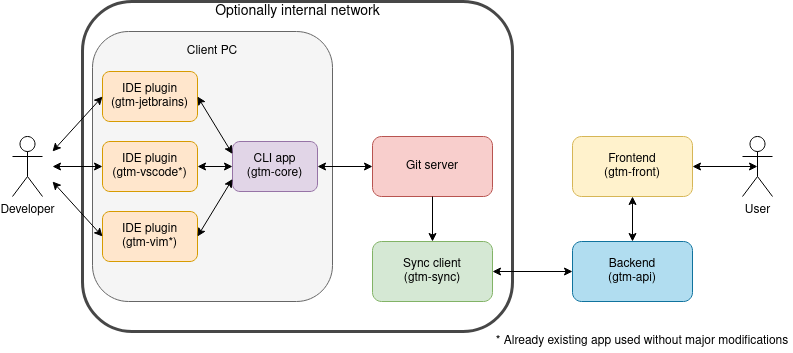
\includegraphics[width=\textwidth]{figures/project_archidecture}
    \caption{Application general design}
    \label{fig:project-archidecture}
\end{figure}

The general time-tracking application can be divided into three different kinds of smaller applications:
\begin{enumerate}
    \item \textbf{Applications that are responsible for data collecting.} These applications are CLI app and IDE plugins and are installed on the developers machine.
    \item \textbf{Applications that are responsible for syncing data.} This role is filled by a Sync client.
    These applications can be installed onto companies/universities servers where they can access Git's internal network if needed.
    \item \textbf{Applications that are responsible for analysing and displaying data.} These are Frontend and Backend apps that are installed on any server.
\end{enumerate}

The reasoning behind this architecture is security and scalability.
For every backend there can be multiple Sync clients all installed on different machines and with different Git access rights.
For every Sync client, there can be multiple client apps all logging time independent of one another.
And in the end, there can be multiple IDE plugins interacting with CLI app.

For security, it is very important to ensure, that no sensitive information is leaked.
To deal with this issue many companies have their Git available only in an internal network.
Not to raise any more security concerns we decided to follow the same principle and not export any Git code outside an internal network.
That is the reason, why Sync client is needed as it has access to the internal network, but only uploads time-tracking related information to our backend.
Therefore, actual code never leaves the internal network.

All the applications that are installed on either client machine or client's server are open source so that the client can easily verify,
they only do what they are meant to do and perform no malicious activities.

To properly manage numerous apps in different programming languages we decided to have each app source code in a separate Git repository.
This reduces the number of merge conflicts and also makes building CI/CD easier.


\section{Client CLI app}\label{sec:cli-app}
%TODO(Tavo): We should somewhere state what are gtm-core, gtm-api, gtm-*
This is the main app on the client machine.
The app is responsible for storing events sent by an editor to files and then later also combining the stored information into Git Note.
You can also see all main stats, such as time spent on a commit via CLI app.

The app is based on open source time tracking app \href{https://github.com/git-time-metric/gtm}{Git-Time-Metric} written in Go and licensed under MIT licence.
We decided to base our app on Git-Time-Metric solution because their app was working the way we wanted to, it had plenty of users meaning plenty of testing done,
and the Git-Time-Metric app had a good code style.

Gtm-core folder structure is displayed in Table
\ref{tab:gtm-core-folder-structure}.

\begin{table}[h]
    \centering
    \begin{tabular}{ | p{3cm} | p{10cm} |}
        \hline
        \textbf{Folder} & \textbf{Purpose}\\
        \hline
        .github & Github related files (Workflows for CI/CD, issues and pull requests templates)\\
        \hline
        deploy & Deploying related files.
        Currently, only Windows installer files and Licence packed with installer.\\
        \hline
        command & Every command has files \textit{<command>.go} and \textit{<command>\_test.go} which respectively are controller for command, and it's tests.
        The controller is responsible for parsing arguments, calling appropriate services and printing out results.\\
        \hline
        docs & Documentation files.\\
        \hline
        epoch & Unix epoch helper functions and their tests.\\
        \hline
        event & Events files serialization and deserialization related services and tests.\\
        \hline
        metric & Metric file serialization, deserialization services and tests.
        Metric files are used for storing time data of files added to Git, but not committed.\\
        \hline
        note & Git notes serialization, deserialization and tests.\\
        \hline
        project & Gtm initialization and uninitialization related services with tests.
        These services are responsible for calling appropriate functions from \textit{scm} package to Git hooks and modifying Git config.\\
        \hline
        report & Report generation services used by report command.\\
        \hline
        scm & Git related services.
        These services are used to wrap \textit{libgit2-go} services into more usable form.\\
        \hline
        test & Python files for running stress tests for gtm-core.\\
        \hline
        util & Various string, date, time and math helper functions.\\
        \hline
        vendor & Directory containing dependencies listed in Git submodules.\\
        \hline
        <root> & Program entry point, Git related files, README and Gofmt style lint configuration .\\
        \hline
    \end{tabular}
    \caption{Gtm-core folder structure.}
    \label{tab:gtm-core-folder-structure}
\end{table}

Although the app was already working we still needed to do many bug fixes and add some features it didn't have.
The biggest change in design was that we moved copied in dependencies to Git submodules.
Although this seems like a small step, it turned out to be very complex to build Go app linked with C library dynamically.
As we didn't manage to get all Git submodules dependencies to properly work in Windows environments
we decided to leave it separately fetched and built in CI/CD workflow file.
Nonetheless, all "snapshot" dependencies were removed.
We also added stress tests to verify the effect of using gtm-core with large amounts of commits.

\section{IDE plugins}\label{sec:ide-plugins}
IDE plugins are installed on developer IDE, and they execute CLI app commands on specific editor events.
Plugins are needed to listen for editor events such as typing without having to give CLI app extensive permissions to run in background.
They also provide a simple way to display some information in IDE.
For example, time since the last commit is shown to the user inside IDE.

Currently, we only have one plugin that is compatible with all Jetbrains IDE's.
The gtm-jetbrains plugin is written in Kotlin and uploaded to Jetbrains plugin repository so that you can easily install it in your Jetbrains IDE.
Kotlin was chosen as the plugin was limited to Java Virtual Machine (JVM) based language and only Java and Kotlin were widely supported.
We have experience in both Java and Kotlin, but we both preferred Kotlin to Java due to its null safety and functional patterns.

Gtm-jetbrains folder structure is described in Table
\ref{tab:gtm-jetbrains-folder-structure}.
Namespace \textit{ee.developest.gtm} is shortened to \textit{<ns>} for readability.

\begin{table}[h]
    \centering
    \begin{tabular}{ | p{3cm} | p{10cm} |}
        \hline
        \textbf{Folder} & \textbf{Purpose}\\
        \hline
        .gradle & Gradle related files\\
        \hline
        src/<ns>/listener & Editor event listeners.\\
        \hline
        src/<ns>/popup & Pop-ups related controllers.
        Used for getting user input\\
        \hline
        src/<ns>/service & Service files such as ConfigService.kt\\
        \hline
        src/<ns>/widget & Widget factories used to display time since last commit and some feedback about initialization.\\
        \hline
        src/<ns> & Gtm-core wrapper used to forward commands from listeners to gtm-core and gtm-core to popup / widget.\\
        \hline
        <root> & Gradle configuration, README and LICENCE.\\
        \hline
    \end{tabular}
    \caption{Gtm-jetbrains folder structure.}
    \label{tab:gtm-jetbrains-folder-structure}
\end{table}

\section{Sync client}\label{sec:sync-client}
Sync client is run on a network, where it can access Git repositories.
On Git push, Git webhook sends a request to gtm-sync via HTTP request.
Then gtm-sync fetches Git repository with its time data, extracts required data and syncs it up to Backend.

The gtm-sync application was written in Rust as it had a more up-to-date library for \textit{libgit2} than both Java and Go, required for interacting with git.
Although we did not have prior experience with Rust we preferred it to C/C++ as it is memory safe and it has higher-level libraries that can be
used for building a web server and API client.
Python and NodeJS that also provide convenient higher-level functions were ruled out because they produce very
big memory footprint compared to Rust, and they also run a lot slower.
Neither of them also gives a type safety that was a must for us.

For the code design, we followed domain-based architecture.
Folder structure for gtm-sync is displayed in Table~\ref{tab:gtm-sync-folder-structure}.

\begin{table}[h]
    \centering
    \begin{tabular}{ | p{3cm} | p{10cm} |}
        \hline
        \textbf{Folder} & \textbf{Purpose}\\
        \hline
        .github & Github workflows.\\
        \hline
        src/config & Config serialization, deserialization and config helper functions.\\
        \hline
        src/gtm & GTM notes parsing and Git related services.\\
        \hline
        src/repo & Tracked repository managing services.\\
        \hline
        src/server & Rocket controllers used for IO.\\
        \hline
        src/sync & Syncing data with gtm-api related services.\\
        \hline
        <root> & Git related files, Cargo package manager files, README and LICENCE.\\
        \hline
    \end{tabular}
    \caption{Gtm-sync folder structure.}
    \label{tab:gtm-sync-folder-structure}
\end{table}

\section{Backend}\label{sec:backend}
Backend is a collection of code that runs on the server.
It receives requests from clients and sends appropriate data back to the clients based on the business logic.
Backend also has a database that stores all the necessary data for the application.

In our case backend receives data from the sync client via REST API requests and stores the data in the database.
End users can interact with the backend though frontend via REST API requests.
%TODO: Kas peaks märkima, et paar endpointi (sync omad) on ka token authiga n-ö programmidele kättesaadavad?

Backend application has been built with Rust programming language using Rocket framework.
Rust is a relatively new low-level statically-typed programming language that's focused on performance and safety.
It gives almost the same speed as C, but guarantees both memory and thread-safety.
It also follows many more functional patterns than Java/C/C++/Go which makes writing code easier and safer once mastered.
Since we needed a fast backend with minimal overhead for processing large datasets Rust was the best choice.
Java, C/C++ and GO were also considered, but the lightweightness of Rust overweights Java whilst memory safety overweights C/C++.
Since Rust was chosen for sync client we decided to choose it for the backend as well.

\subsection{Backend design}\label{subsec:backend-design}
Backend code base has been built following Domain Driven Design (DDD).
DDD is a concept that centers the development and code structure around the business domain.
It helps to keep the code more organized, maintainable and extendable~\cite{domain-driven-design}.
% TODO: More explanation for DDD, some reference

A layered architecture can be found on Figure~\ref{fig:backend-layered-diagram}.
\begin{figure}[H]
    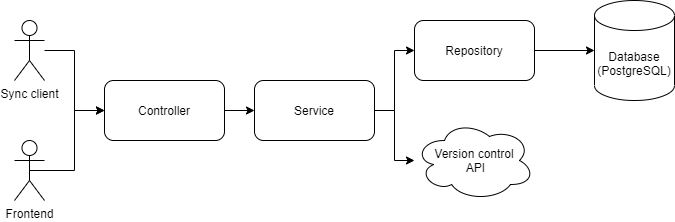
\includegraphics[width=\textwidth]{figures/backend_layered_diagram}
    \caption{Backend architecture}
    \label{fig:backend-layered-diagram}
\end{figure}

Folder structure is displayed in Table~\ref{tab:gtm-api-folder-structure}.
\begin{table}[h]
    \centering
    \begin{tabular}{ | p{3cm} | p{10cm} |}
        \hline
        \textbf{Folder} & \textbf{Purpose}\\
        \hline
        .github & CI/CD related files\\
        \hline
        migrations & Migrations for Diesel. \\
        \hline
        src/common & Widely used files.\\
        \hline
        src/db & General database connection.\\
        \hline
        src/domain & Main business logic.\\
        \hline
        src/security & Authentication and authorization.\\
        \hline
        src/vcs & Version control.\\
        \hline
        <root> & Configurations, README and LICENCE.\\
        \hline
    \end{tabular}
    \caption{Gtm-api folder structure.}
    \label{tab:gtm-api-folder-structure}
\end{table}

\subsection{Database design}\label{subsec:database-design}
One requirement when choosing the database was that we needed it to have bindings for our Object-relational mapper (ORM),
so we could easily use it in our application.
This requirement narrowed the search down to SQLite, MySQL and PostgreSQL as they were the only languages with full support in Diesel.
There are other ORM-s written for Rust, but Diesel is one of the most popular ones, so we decided to go with it as
there was no need to use some other database.
% TODO: S6nastus paremaks

SQLite was ruled out as it is not strongly typed, and it does not have the same amount of features PostgreSQL and MySQL have.
For choosing between MySQL and PostgreSQL it came down to personal preference as both of them are strongly typed and
support all the required features, including recursive queries.
Both of them are also open source.

We decided to go with PostgreSQL as we had prior experience with it.

As we are running the application in "beta", we decided to run the database in a docker container on our development machine to
reduce the cost of upkeep.
For data persistence, we have mounted database files volume to host machine.

\subsubsection{Database versioning}\label{subsubsec:database-versioning}
As we have users data in our database it is important to also persist it through database schema updates.
For this, we use migrations and let Diesel handle the updates.
Every time database change is required, we add new migration with both up and down scripts that can be used by Diesel
to run the migration or revert it.
Diesel is configured to automatically run updates added to the release.
As reverting database changes can result in a loss of data, it has to be done manually via Diesel CLI app.

\subsubsection{ERD Schema}\label{subsubsec:erd-schema}
The database holds data about tracked time, registered users and how the users can access time data.
The structure of the database schema is described in Figures~\ref{fig:erd-schema-user} and~\ref{fig:erd-schema-general}.

Time data follows the structure of the Git commits tree and file tree.
The \textit{repositories} table contains general information about the Git repository such as name and the sync client
responsible for tracking it.
Then the \textit{commits} table has the information about commits such as author, timestamp and commit message.
Each \textit{commits} table entry also has a reference to the repository it is committed to.
Every commit has zero or more files that were edited in it.
These files are contained in \textit{files} table, and they contain information about files added and deleted.
To have more accurate data about when the time was spent separate table is needed as there is no guarantee that
the time spent editing files is spent just before the commit timestamp.
For this, we have a table called \textit{timeline} which olds timestamps and durations of every consecutive edit as
well as a reference to a file in which the time was spent.

The \textit{users} and \textit{roles} table are responsible for persisting user login credentials, roles and connected OAuth accounts.
As we allow the user to optionally register only via OAuth, the password field is nullable.
Users that have no password can only log in via OAuth, but they can also add a password at any time.

Every user can have multiple rows with role \textit{USER} being added to every user by default.
There are three roles in total: \textit{USER}, \textit{LECTURER} and \textit{ADMIN}.
Currently, there are no rules in the database for any of the roles which means all checks are done in software.
More detailed description about roles can be found in~\nameref{subsec:roles} subsection.

Every user also has zero or more OAuth logins stored in \textit{logins} table.
There is a limit that every user can have at maximum one OAuth login per login type.
If one already exists, it is updated instead of adding new.

User emails retrieved from OAuth providers are stored in \textit{emails} table to avoid unnecessary web requests.

\begin{figure}[H]
    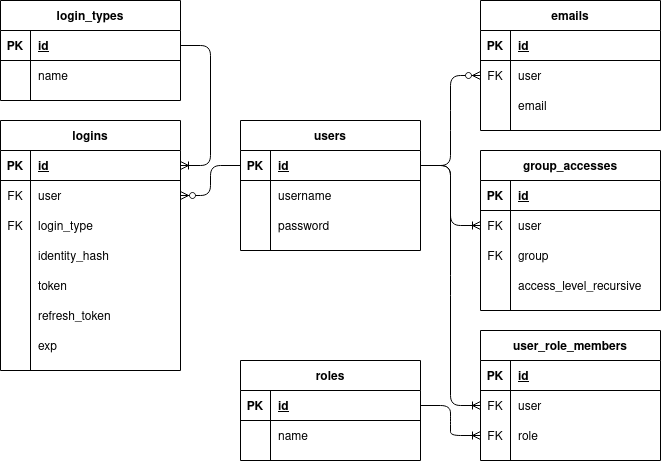
\includegraphics[width=\textwidth]{figures/erd_schema_user}
    \caption{ERD schema for user related tables}
    \label{fig:erd-schema-user}
\end{figure}

\begin{figure}[H]
    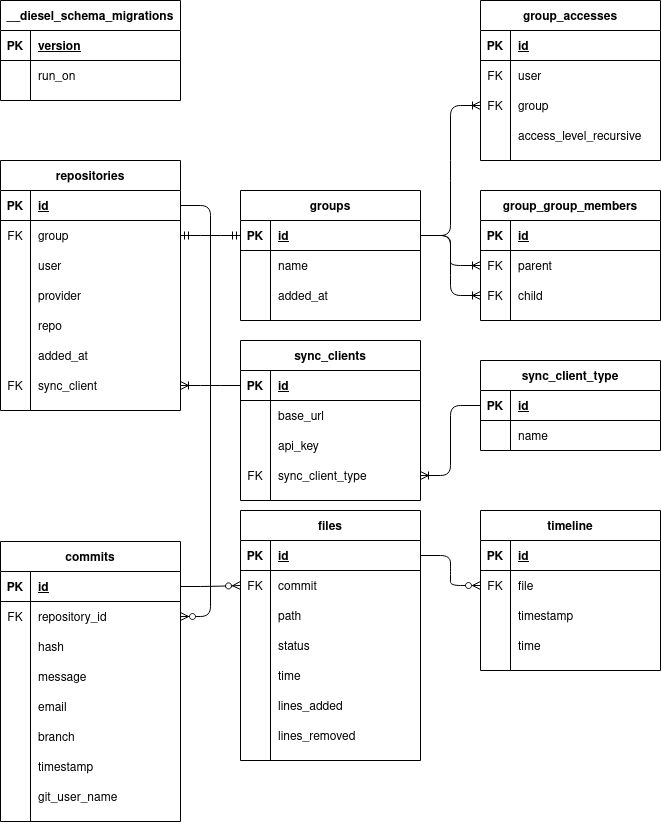
\includegraphics[width=\textwidth]{figures/erd_schema_general}
    \caption{ERD schema for non-user related tables}
    \label{fig:erd-schema-general}
\end{figure}

\section{Frontend}\label{sec:frontend}
A frontend is a software program or website that the user interacts with.
In our case frontend is a website where the user can see time tracking data according to the privileges.
Although technically also CLI app can be considered frontend, when we refer to frontend we only mean the website.

The frontend has been build using ReactJS library.
According to the State of Frontend 2020 report, ReactJS is the most used JavaScript framework and also the framework which developers want to learn or keep using the most.
It is faster than Angular, and its somewhat functional style was more pealing for us than the style of Vue.
It was chosen by Marten, who's mostly responsible for frontend development and had some prior experience with it.
Most popular frontend frameworks by popularity are shown in Figure~\ref{fig:frontend-framework-popularity}.

\begin{figure}[h]
    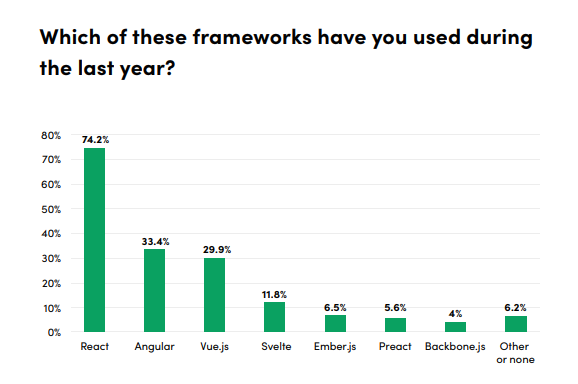
\includegraphics[width=\textwidth]{figures/frontend_framework_popularity}
    \caption{Frontend framework popularity~\cite{state-of-frontend-report}}
    \label{fig:frontend-framework-popularity}
\end{figure}

\subsection{Code design}\label{subsec:code-design}
Frontend code is written following the main principles promoted by ReactJS community and documentation.
For an example component's names use \textit{PascalCase}, helper files use \textit{camelCase}, folders use \textit{camelCase}.
Code is divided into multiple files/components to prevent code repetition, inline CSS is avoided, the liner is used to make code easier to use, service calls are in the separate file, etc.
To improve code quality and readability TypeScript was chosen as it is a strongly typed language which JavaScript is not.
This decision was not made at the beginning of the project but as the code kept growing and readability suffered the decision was made.
One of the biggest reasons to switch from JavaScript to TypeScript was that due to being a strongly typed language,
TypeScript has better IDE support.
Folder structure is displayed in Table
\ref{tab:gtm-front-folder-structure}.

\begin{table}[h]
    \centering
    \begin{tabular}{ | p{3cm} | p{10cm} |}
        \hline
        \textbf{Folder} & \textbf{Purpose}\\
        \hline
        .github & CI/CD related files\\
        \hline
        src/api & Service calls .\\
        \hline
        src/assets & Images and icons. \\
        \hline
        src/containers & Main container structure (Header, Footer, Content, etc.)\\
        \hline
        src/models & Easy-Peasy state management models.\\
        \hline
        src/reusable & components that can be reused.\\
        \hline
        src/routes & Routes.\\
        \hline
        src/scss & Style.\\
        \hline
        src/store & Store for state management.\\
        \hline
        src/utils & Helpers.\\
        \hline
        src/views & Views that are used once.\\
        \hline
        <root> & TypeScript configuration, package.json, README and LICENCE.\\
        \hline
    \end{tabular}
    \caption{Gtm-front folder structure.}
    \label{tab:gtm-front-folder-structure}
\end{table}

\subsection{User interface design}\label{subsec:user-interface-design}
User interface must be built keeping user in mind.
User experience is the most important part of a web application.
If the user does not have a good experience with the interface, it might be the end of the interaction between the user and the application.
Since the team did not have any professional designers, CoreUI was a great choice to make the design process much easier.
CoreUI is an Open Source Bootstrap Admin Template which is built on Bootstrap and written with readability in mind.
The design and easy usability were the decisive factors in choosing CoreUI.

However, CoreUI's charts were not customizable to the extent we required.
For better customization, Recharts was chosen for building graphics.
Recharts is a composable charting library built on React components and D3.
It is much more customizable than CoreUI charts as it allows combining different bar charts, line charts, etc.
\cite{recharts-readme}

At this point, the design problem arose again.
Designing graphs were done in the following manner:
\begin{enumerate}
    \item Understand the functionality and create an initial component.
    \item Let it settle for some time and then discuss with the team.
    \item Finalize component and release it for test users.
    \item Make final changes according to the users' feedback.
\end{enumerate}
Design patterns such as graph sizes, colours, spacings, fonts etc. were chosen in such a way that they would look similar to CoreUI graphs.

\subsection{State management}\label{subsec:state-management}
State management does not have a certain winner.
Choosing a state management library comes down to personal preference.
We decided to use Easy-Peasy which is built on the most popular state management library Redux.
Easy Peasy was chosen over Redux because Redux has a steep learning curve but Easy-Peasy is easy to use.
%TODO: Vb contents alla?


    \chapter{Project contents}\label{ch:project-contents}
    \section{CLI app}\label{sec:cli-app-contents}

\subsection{CLI app improvements}\label{subsec:cli-app-improvements}
Our CLI app is based on~\nameref{subsec:git-time-metric}, an already working open source time tracking app.
Although it already had all the basic features, some improvements and fixes were required.

Firstly \textit{--cwd=\{some/path\}} option was added to allow easier integration of plugins.
Option to pass a current directory as an option is required, as IDEs not launched from terminal sometimes have their working
directory elsewhere and setting custom working directory every time we call CLI app is more complicated than passing an argument.

To clean up user home directories, global configuration files were moved from \textit{~/.git-time-metrics/} to \textit{~/.config/gtm/}.
For Windows, a new installer was built to make installing easier.
Also, it was chosen to switch from statically compiling SSH2 Libraries into our application to dynamic linking.
For Debian Linux, a build script for Debian packages was set up to also provide Debian packages with every release.

The application was updated to automatically add a fetch refspecs to fetch data from remotes on Git fetch.
Also, a pre-push Git hook was added to automatically push data to origin.
With these two hooks, the time data is automatically fetched pushed whenever Git push is made requiring the user no extra effort.

To still allow users to only track time locally, a \textit{--local} option was added to \textit{init} command.
Also, \textit{--auto-log=[jira|gitlab]} option was added to support automatic time logging to commit messages.
Currently, this time can only be collected in Jira, but there is also and \href{https://gitlab.com/gitlab-org/gitlab/-/issues/16543}{issue}
open for Gitlab to implement this.\cite{gitlab-time-issue}

To allow filtering data by branch name we decided to also store the current branch name in Git Notes when committing a file.
This couldn't be avoided because the branch is simply a pointer to commit and there is no guarantee that this pointer isn't changed or deleted.

For students, it is important to view time spent on specific tasks.
In most subjects, the tasks are placed in separate subdirectories for better file management.
To allow users to view time spent on specific tasks, a \textit{--subdir="sub/dir/name"} option was added to filter out
data based on directories.

Although Git supports automatic merging/rewriting of the notes, it was inconsistent in some cases, especially when the user
wants to also rewrite manually added notes.
To keep time data after Git rebases, a new command \textit{rewrite} was introduced.
This command is run by Git post-rewrite hook, and it rewrites notes so that they still point to the correct commit.

\subsection{Initializing tracking}\label{subsec:init-tracking}
Main flow for initializing tracking for repository is described in Figure~\ref{fig:init-tracking}.
\begin{figure}[h]
    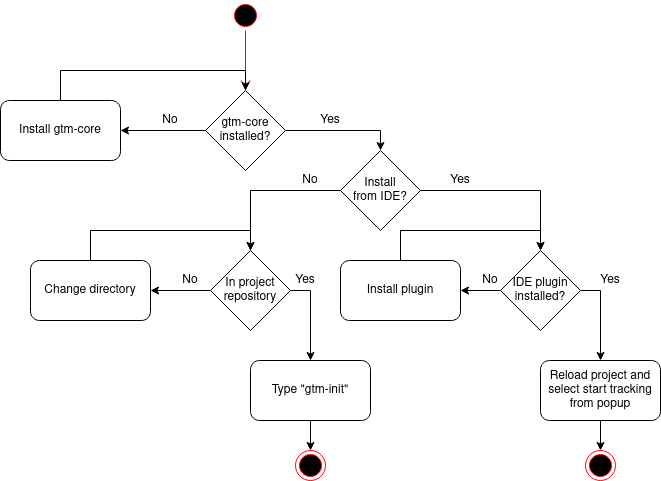
\includegraphics[width=\textwidth]{figures/init_tracking}
    \caption{Initialize tracking}
    \label{fig:init-tracking}
\end{figure}

The first requirement is that you need to have gtm-core installed and added to \textit{PATH} in order to initialize tracking.
If the user has gtm-core installed, he can initialize tracking from command line.
To do that, it is required to change your current directory to be somewhere within Git root directory.
Time tracking is then initialized with \textit{gtm init} command.
The command supports following arguments:

\begin{table}[h]
    \centering
    \begin{tabular}{ | p{3cm} | p{10cm} |}
        \hline
        \textbf{Argument} & \textbf{Description}\\
        \hline
        \textit{--terminal} & Enable time tracking for terminal. (Requires terminal plugin)\\
        \hline
        \textit{--auto-log} & Either \textit{gitlab} or \textit{jira} to automatically log time
        into commit messages with given format.\\
        \hline
        \textit{--local} & If set, no Git fetch nor push hooks are added.
        Time data is only stored locally.\\
        \hline
        \textit{--tags} & Optionally add tags to project for better local organization.\\
        \hline
        \textit{--clear-tags} & If project already has some tags running it with given flag removes previously added flags.\\
        \hline
        \textit{--cwd} & Useful for specifying working directory for scripts.\\
        \hline
    \end{tabular}
    \caption{Gtm-front folder structure.}
    \label{tab:gtm-init}
\end{table}
It is safe to run \textit{gtm init} multiple times with any of the arguments.

The user can also initialize time tracking from within IDE if he has GTM plugin installed.
Currently, only Jetbrains IDE plugin supports starting tracking.
To initialize time tracking from Jetbrains IDE the user needs to open/reload the project he wishes to add time tracking to.
Upon doing that he is prompted to choose whether to start tracking or not.
To initialize tracking, start tracking has to be chosen.
This initializes tracking for the currently open repository with default settings (equal to no argument for CLI).
If the user chooses not to initialize tracking, his choice is persisted in a local Jetbrains project config file within \textit{.idea} directory.
To later add tracking to a repository, he needs to do it from the command line or by deleting the Jetbrains' project settings file.


\section{IDE Plugins}\label{sec:plugins}

IDE plugins are used to capture editor-specific events and then execute appropriate commands on gtm-core.
Basically gtm-core and IDE plugin combo works like a language server and code formatting plugin combo.
This eliminates the need to write duplicate code when writing plugins for multiple IDEs.
Currently, we have full support for Jetbrains and some support for Vim.
There are also many more plugins that have been previously written for original Git-Time-Metric, and most of them also work with our app.

\subsection{Jetbrains}\label{subsec:jetbrains-plugin}
Jetbrains also had a plugin for the original Git-Time-Metric, but the IDE has gone through lots of changes since the last update to the plugin.
As of 2021, this causes Jetbrains IDEs to crash.
We decided to fully rewrite the plugin as it heavily used now deprecated Jetbrains components.

The plugin catches following events and forwards the data to gtm-core:
\begin{enumerate}
    \item Opening the file in the editor.
    \item A mouse pressed inside the editor (on file).
    \item A process run (Mostly build, test, debug or run, but can be any other process you run via IDE)
    \item File saved.
    \item Visible area changed (Window resized / split).
\end{enumerate}

In response, the plugin gets the time since the last commit (uncommitted time), which it shows on the bottom status bar.

In addition to silently listening for events and updating time, the plugin communicates with the user via pop-up dialog and notification.
The pop-up dialog is used to prompt the user whether he wants to start tracking time for the project as described in~\nameref{subsec:init-tracking}
Notifications are used to report errors and more important action results (such as whether adding tracking was successful).

\subsection{Vim}\label{subsec:vim-plugin}
An already existing \href{https://github.com/git-time-metric/gtm-vim-plugin}{plugin} for vim was forked as it had all the required features.
Version numbers and update links were changed to comply with our version.
As the Vim script file to give the support for tracking time and also displaying it on the status line is under 80 lines long
it perfectly describes, why it was necessary to have gtm-core as a separate program instead of writing the business logic inside the plugin.


\subsection{Adding tracking to repositories}\label{subsec:adding-tracking}
We have added three levels to view time data:
\begin{enumerate}
    \item Add tracking (locally), view data via GTM CLI app.
    \item Add tracking (locally), log data to commit messages.
    \item Add tracking, sync data to GTM Web App.
\end{enumerate}

All smaller level features can be included while using a higher level option.
Viewing data via CLI app is always possible, as it is the same app that is responsible for recording data.
This can be done both only locally or with pushing and pulling notes from remotes.
You can also add logging time spent to commit messages in both of the scenarios as it simply works on top of the already
existing system and only modifies the commit message.
To use auto logging option you simply need to add \textit{--auto-log=[gitlab|jira]} option when initiating tracking. % for a repository.

To view data from the web interface, some more steps are required.
User flow for making repository visible on GTM web application is shown in Figure~\ref{fig:add-tracking-user-flow}.

\begin{figure}[h]
    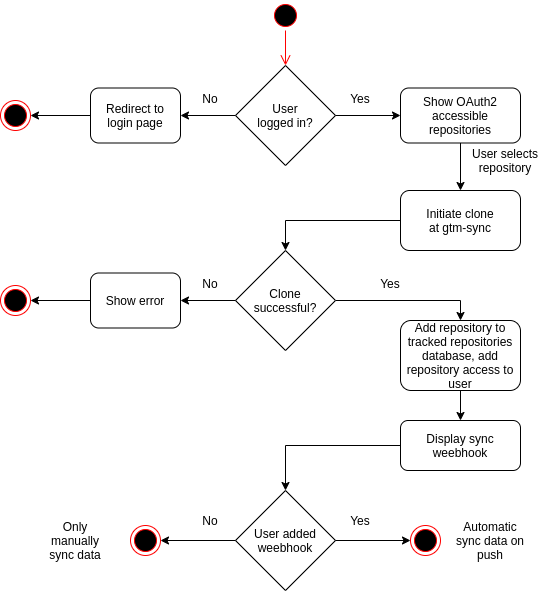
\includegraphics[width=\textwidth]{figures/add_repo_user_flow}
    \caption{Add tracking user flow}
    \label{fig:add-tracking-user-flow}
\end{figure}

Firstly, to have our sync client access the data, you cannot have time data only stored locally.
Then to add a repository, you need to have linked appropriate Git server provider account via OAuth so that we can
verify that you have the access to the repository.
After that, you need to search for the repository from the web interface and click \textit{"Start tracking"} button.
With that, the tracking is technically added, but to also automatically sync time data on every push to remote,
you also need to add a webhook.

To make sure that the repository can be accessed by the user the request to an appropriate provider is made again
when user has pressed \textit{"Start tracking"} button.
This check is required as the user could easily guess other peoples private repository clone URLs and then post
it to our backend with his own JWT.
This extra check also means you cannot add tracking to self-hosted Git servers that do not provide OAuth2.
However, we could not find any better way to identify that the given user has access to some Git repository and
therefore it was decided to not support any custom setups.

\section{Sync client}\label{sec:sync-client-content}
Sync client is used for fetching data from Git notes and then syncing it up to the backend.
The gtm-sync application is configured in a local configuration file, and it exposes some REST API endpoints
that allow adding new repositories and endpoints for triggering syncing process

Manually editing configuration is meant for a developer as it gives more control over application and REST API is
for machine to machine communication.
All the API endpoints are described in Table~\ref{tab:gtm-sync-endpoints}.

\begin{table}[H]
    \centering
    \begin{tabular}{ | p{8cm} | p{6cm} |}
        \hline
        \textbf{Endpoint} & \textbf{Description}\\
        \hline
        GET /repositories/<provider>/<user>/<repo> & Used to get data about single repository \\
        \hline
        POST /repositories & Used to start tracking repository\\
        \hline
        GET /repositories/sync-all & Used to sync all tracked repositories to backend\\
        \hline
        GET/POST /repositories/<provider>/<user>
        /<repo>/sync & Sync single repository.
        Post is allowed as webhooks sometimes only support post requests\\
        \hline
        POST /hooks/github/push & Endpoint for Github hook to sync repository\\
        \hline
        POST /hooks/gitlab/push & Endpoint for Gitlab hook to sync repository\\
        \hline
    \end{tabular}
    \caption{Gtm-sync API endpoints.}
    \label{tab:gtm-sync-endpoints}
\end{table}

For configuration \textit{config.toml} file is used.
It contains information about the backend, where to sync data, Git user authorization (SSH keys), and about tracked repositories.
Although gtm-sync supports cloning with both Secure Shell Protocol (SSH) and HTTPS, we have limited it to HTTPS in our backend for simplicity.
In order for SSH keys to work, we have created a user called \textit{gtm-user} to TalTech Gitlab server and added an SSH key to him.
This means \textit{gtm-user} has to have at minimal reporter access to the project in order to track it.
For GitHub and GitLab we only support tracking public repositories for now and for the SSH cloning to work, the SSH key was added to
Tavo Annus'es personal account.
The configuration variables are described in Table~\ref{tab:gtm-sync-config}.

\begin{table}[H]
    \centering
    \begin{tabular}{ | p{6cm} | p{6cm} |}
        \hline
        \textbf{Variable} & \textbf{Description}\\
        \hline
        target\_base\_url & Backend URL, used for syncing data \\
        \hline
        sync\_base\_url &  Public URL to self (Optional), used to force sync\\
        \hline
        access\_token & Backend API key\\
        \hline
        ssh\_public\_key & Path to Git user public ssh key\\
        \hline
        ssh\_private\_key & Path to Git user private ssh key\\
        \hline
        repositories\_base\_path & Path to store cloned repositories at\\
        \hline
        repositories & List of tracked repositories (each has path in filesystem and clone URL)\\
        \hline
    \end{tabular}
    \caption{Gtm-sync config variables.}
    \label{tab:gtm-sync-config}
\end{table}

\section{Backend}\label{sec:backend-content}
Backend is the central part of our system as it connects frontend, sync client, and database.
It communicates with gtm-sync and gtm-front via REST API requests.

Sync client which has API key registered has access to the endpoints in Table~\ref{tab:gtm-api-endpoints-for-sync}.
\begin{table}[H]
    \centering
    \begin{tabular}{ | p{5cm} | p{4cm} | p{5cm} |}
        \hline
        \textbf{Endpoint} & \textbf{Parameters} & \textbf{Description}\\
        \hline
        POST /repositories & - & Sync client can send new repo timeline data \\
        \hline
        PUT /repositories & - & Sync client can send existing repo updated timeline data\\
        \hline
        GET /commits/hash & provider: string, user: string, repo: string & Returns last commit hash, timestamp and tracked commit hashes\\
        \hline
    \end{tabular}
    \caption{Gtm-api endpoints for sync client.}
    \label{tab:gtm-api-endpoints-for-sync}
\end{table}

An authorized user has access to the endpoints in Table~\ref{tab:gtm-api-endpoints-secured}.
\begin{table}[H]
    \centering
    \begin{tabular}{ | p{5cm} | p{4cm} | p{5cm} |}
        \hline
        \textbf{Endpoint} & \textbf{Parameters} & \textbf{Description}\\
        \hline
        GET /groups & - & Returns all the groups logged-in user has access to. \\
        \hline
        GET /\{group\_name\}/activity & start: int, end: int, interval: string, timezone: string & Returns activity for group. \\
        \hline
        GET /\{group\_name\}/subdirs-timeline & start: int, end: int, interval: string, timezone: string, depth: int & Returns sub-directory timeline for group. \\
        \hline
        GET /\{group\_name\}/timeline & start: int, end: int, interval: string, timezone: string & Returns timeline for group. \\
        \hline
        GET /groups/\{group\_name\}/stats & start: int, end: int, depth: int & Used to get group stats for leaderboard view.\\
        \hline
    \end{tabular}
    \caption{Gtm-api secured public endpoints}
    \label{tab:gtm-api-endpoints-secured}
\end{table}

Unauthorized user has access to the endpoints in Table~\ref{tab:gtm-api-endpoints-public}.
\begin{table}[H]
    \centering
    \begin{tabular}{ | p{5cm} | p{4cm} | p{5cm} |}
        \hline
        \textbf{Endpoint} & \textbf{Parameters} & \textbf{Description}\\
        \hline
        POST /auth/login & - & For login \\
        \hline
        POST /auth/register & - & For registering new account \\
        \hline
    \end{tabular}
    \caption{Gtm-api not secured public endpoints.}
    \label{tab:gtm-api-endpoints-public}
\end{table}

All the endpoints can be found \href{https://cs.ttu.ee/services/gtm/api/swagger/index.html}{here}.

\subsection{Security}\label{subsec:scurity}
Our application holds data, that shall not be visible to all clients and therefore some kind of authentication and authorization methods are required.
For the data stored in Git notes, we decided no extra security is required, as the time data isn't more sensitive than the actual code.
The security of source code stored in a Git repository is handled by a client himself and Git providers.
If they wish to have some more protection for Git notes, they can configure it themselves.
We only provide the option to have notes only stored locally (not pushed to origin).

For the web application, we need to implement our own security measures.
For the most basic usage, we have a simple username and password authentication.
Accounts that only have password authentication are not authorized to access any groups nor repositories unless the Admin user
explicitly gives them access to any.

To automatically get access to repositories you are a contributor of you need to authenticate yourself via OAuth2 standard.
This way we can verify, that the user signing in to our application is the same user that has access to some Git repository.

\subsubsection{OAuth2}\label{subsubsec:oauth2}
For OAuth2 authorization rocket{\_}oauth2 library is used, that follows RFC-6749 standard~\cite{rocket-oauth2, oauth2}.
We support authentication via \href{https://github.com/}{Github.com}, \href{https://about.gitlab.com/}{Gitlab.com},
\href{https://bitbucket.org/}{Bitbucket.org}, \href{https://azure.microsoft.com/}{Azure} (Microsoft account) and
TalTech \href{https://gitlab.cs.ttu.ee/}{gitlab server}.
The first three were chosen as they are the most common Git server providers as of 2021.
Authentication via Microsoft was added as TalTech (and also numerous other universities/companies) use it and therefore
all students have already registered accounts there.
Also, it provides access to user emails, that can be later used to filter out user commits.
TalTech Gitlab server was added, as the application is currently developed for TalTech and therefore it was a requirement
that everything shall also work on TalTech Gitlab server.

From all OAuth2 providers at least user read access is required to get access to user emails, which we use to link users with commits.
For OAuth2 providers, which are also a Git server providers also permissions to read user repositories data are required.
User repositories data is used to give user automatically access to his own repositories and also display repositories
not currently tracked by GTM.
It also allows adding automatic data collection to user repositories more easily, as a user can browse through
repositories from different Git server providers.

\subsection{Groups system}\label{subsec:group-system}
One of the requirements for our app was that it should be possible to group repositories together.
The grouping is needed to view statistics for multiple repositories at once and also compare groups of repositories.
The grouping system should be also capable of controlling user access rights to different repositories.

Requirements for the grouping system were:
\begin{itemize}
    \item It shall be possible to group both repositories and groups already consisting of repositories into a bigger group.
    \item Single repository may belong to multiple groups.
    \item Group access can be limited to only viewing summary (group total).
    \item Granting user an access group's subgroups and then removing it shall have no side effects. (Accesses to subgroups shall not be persisted)
\end{itemize}

As the groups may consist of both groups and repositories we decided to automatically create a group for every repository.
This means new groups can only consist of zero or more other groups.
If we need to get the repository we can fetch all the group ids that are accessible and then query from repositories database by
comparing repositories group id against previously fetched ids.
To fetch a group with all of its subgroups a recursive Structured Query Language (SQL) query was needed as the groups'
hierarchy formulates a tree-like structure.
Our database provider PostgreSQL supports recursive queries so there were no technical problems with implementing it on SQL database.
A simplified version of our group system database tables can be seen in Figure~\ref{fig:group-system}.

\begin{figure}[h]
    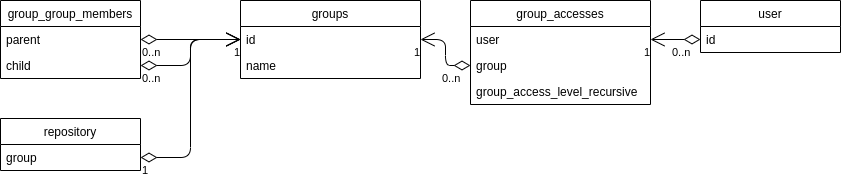
\includegraphics[width=\textwidth]{figures/group_system}
    \caption{Application groups system}
    \label{fig:group-system}
\end{figure}

This tree-like groups hierarchy allows us to easily give and take user access to any group.
If we want to change access from only parent group to also all subgroups access, we can simply toggle access{\_}level{\_}recursive
variable.
If we remove one particular group access, all other accesses remain in place,
meaning that groups previously accessible via some other group access remain accessible via the other group access.

\subsection{Roles}\label{subsec:roles}
Our application has three different roles to control user permissions.
A single user can belong to multiple roles and also new roles can be dynamically added to the database as they are
kept in a separate table.
Currently, there are three roles in total: \textit{USER}, \textit{LECTURER} and \textit{ADMIN}.
Role \textit{USER} is added to every created user, and it has no extra permissions.

People with \textit{USER} role can:
\begin{enumerate}
    \item View data from Git repositories, they have access to.
    \item Add new repositories.
    \item Delete repositories they have access to.
\end{enumerate}

People with \textit{LECTURER} role can:
\begin{enumerate}
    \item View data from Git repositories, they have access to.
    \item Add new repositories.
    \item Delete repositories they have access to.
    \item Give access to others.
\end{enumerate}

People with \textit{ADMIN} role can:
\begin{enumerate}
    \item Assign new roles to other users.
    \item View data from all the repositories and groups.
    \item Give other users group accesses.
\end{enumerate}

\section{Frontend}\label{sec:frontend-content}
Frontend is one-page web application.
Users can log in and see their data according to their privileges.
This application has two main parts - profile and data visualization.
Under profile, users can change password, link OAuth accounts and delete an account and add repositories.
Data visualization is divided into 3 parts - \textit{"Dashboard"}, \textit{"Leaderboard"} and \textit{"Timeline comparison"}.
In those tabs users can see their/others data as graphs and tables.

\subsection{Authentication and authorization}\label{subsec:authentication-and-authorization}
Authentication and authorization is implemented using a bearer token system.
The user gets JSON Web Token (JWT) from API and stores it to the local storage and adds it to every request header.
The user has to log in from \textit{"Log in"} page.
Login page view can be found in Figure~\ref{fig:login}.
On success, client receives JWT from the backend and stores it in local storage.
Then the user is automatically redirected to the main page.
Users can log in with OAuth or username/password.
In case of OAuth is chosen, the user is redirected to according OAuth platform for authentication.
If The authentication is successful, the user is redirected to the frontend with JWT.
JWT is saved on local storage and the user is redirected to the main page where he/she can access their data.
Login and register user flows are described on Figure~\ref{fig:login-signup-diagram}.

\begin{figure}[H]
    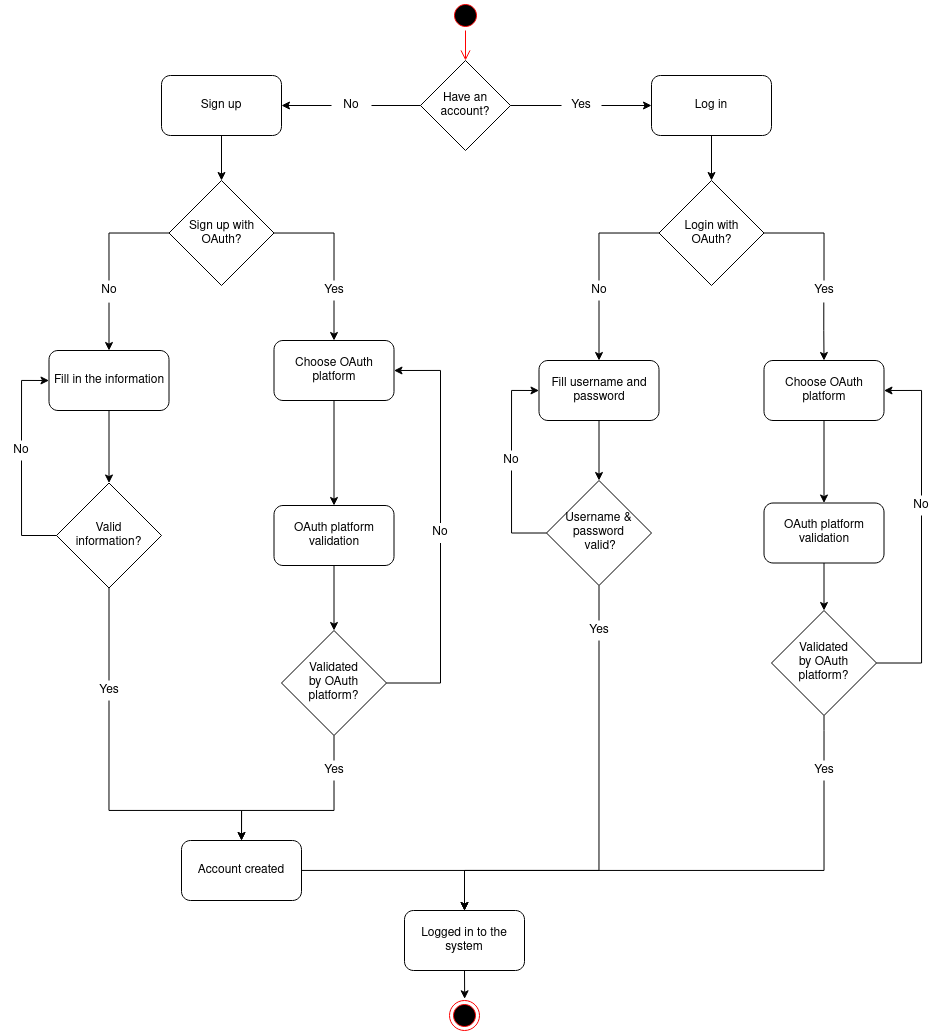
\includegraphics[width=\textwidth]{figures/login_signup_user_flow}
    \caption{Log in and sign up flows}
    \label{fig:login-signup-diagram}
\end{figure}

\subsection{Profile}\label{subsec:profile}
\subsubsection{OAuth linking}\label{subsubsec:oauth-linking}
It is also possible to link multiple OAuth platforms to one account (Figure~\ref{fig:link_accounts}).
In that case, the user has to log in and head to the profile page where he can find the link  under \textit{"Accounts"} tab.
If an account from OAuth platform is already linked then the backend unlinks it from this account, otherwise user is redirected to OAuth platform for authentication.
On success the user will be redirected to the frontend and the user can access new repositories that this OAuth platform account has.
OAuth linking flow is described in Figure
\ref{fig:account-linking}.

\begin{figure}[H]
    \centering
    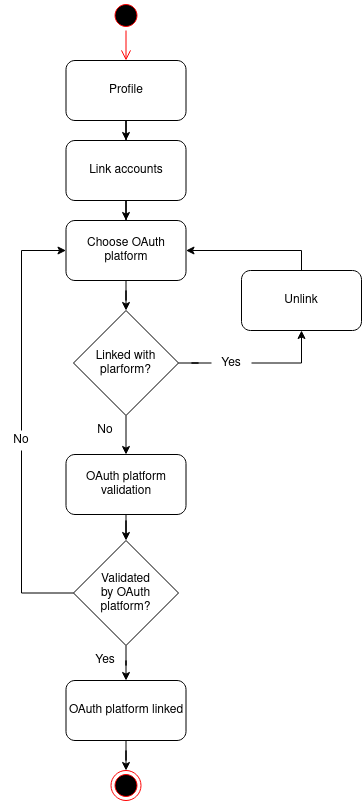
\includegraphics[width=0.5\linewidth]{figures/oauth_linking_user_flow}
    \caption{OAuth linking with user}
    \label{fig:account-linking}
\end{figure}

\subsubsection{Change password}\label{subsubsec:change-password}
Users can also change password (Figure~\ref{fig:change_password}).
In the \textit{"Profile"} view under the \textit{"Change password"} tab user has to fill all the fields correctly and the password will be changed.
If the user does not have a password (OAuth registration), only new password fields have to be filled.
Once you have already added a password, it's not possible to remove it to avoid the possibility to have inaccessible accounts.

\subsubsection{Repositories}\label{subsubsec:repositories}
Under repositories tab user can see all his repositories (Figure~\ref{fig:repositories}).
The user can start tracking a new repository by clicking \textit{"Start tracking"} and then adding a webhook to the according OAuth platform.
If \textit{"Start tracking"} is clicked and everything is successful, a blue info box with instructions for webhook setup will pop up.
In case the user wants to start tracking again then the repository can be found at the end of the list with a button initialize again.
Tracking can also be stopped by clicking on the red button with a trash can.

\subsubsection{Delete account}\label{subsubsec:delete-account}
Account deletion is under \textit{"Delete account"} tab (Figure~\ref{fig:delete_account}).
To keep away accidental account deletion user has to write their name to the input box and then can submit.
If the account is deleted, the user is redirected to the \textit{"Login page"}.
% TODO: Mis siis kui viimase OAuthi unlinkid? ka delete? tegelt vist oleks warning vms parem aga idk

\subsection{Data visualization}\label{subsec:data-visualization}
Data visualization is divided into three pages - dashboard, leaderboard and comparison.
From the sidebar, the user can navigate to the necessary page, and on top of the page user has a selection of properties according to the graphs.

\subsubsection{Dashboard}\label{subsubsec:dashboard}
Dashboard is the main landing page if user is logged in.
\textit{"Dashboard"} view can be found in Figure~\ref{fig:dashboard}.
\textit{"Dashboard"} contains three graphs and inputs.
From inputs, the user can change group, time period and interval.
User can choose between all the groups he/she has access to.
The time period has start and end which cannot be apart more than a year for performance reasons.
Intervals are days, weeks and months.

The first graph is a combination of a line and a bar charts, which describes time spent writing code in a period of time and also shows how many users were active at the interval.
The X-axis shows the period of time and Y-axis shows the time spent during the period.
The Y-axis also shows active users count during the period.
The line shows time spent and bar shows users count.

The second graph is a line chart which describes activity hours during the chosen period.
According to the interval, it shows daily activity, weekly activity or monthly activity.
The X-axis shows interval over selected time period, and the Y-axis shows an average time spent during each interval.
If the interval is day then the X-axis describes each hour, in case it is a week, the X-axis describes each week day, etc.
The Y-axis also shows lines added and removed from code.
This graph brings out the time frame when users are actively programming.

The third graph is a bar chart that describes time spent in folders or files.
The X-axis shows the time period, and the Y-axis shows the time spent during day/week/month depending on the chosen interval.
Bars are stacked on each other and each bar describes one folder or file.
This graph brings out on which tasks people spend most of their time on and is very useful for lecturers who want to see which homeworks take more time.
The depth of how far into files tree the app goes to group files is set to 2, as this makes
it usable for most of the subjects.
It will be made configurable in the future.

\subsubsection{Leaderboard}\label{subsubsec:leaderboard}
Leaderboard contains four inputs and two tables where users and files/folders can be easily compared.
\textit{"Leaderboard"} view can be found in Figure~\ref{fig:leaderboard}.
Inputs contain group selection, date selection and depth selection.
Depth determines how deep will the search go for files and folders.

The first table shows info about users in the chosen group.
Data is divided into 7 columns - total time, commits, lines added, lines removed, lines per hour, commits per hour and lines per commit.
By clicking on the column header the contents of the table will be sorted accordingly.

The second table shows info about the project(s) file system.
Data is divided into 8 columns - total time, commits, lines added, lines removed, lines per hour, commits per hour, lines per commit and users.
The sequence can also be changed by clicking on the column header.
This table can be useful for comparing different tasks in university as they are usually placed in separate folders.

At the end of the page, there is an export data button that allows downloading Comma Separated Values (CSV) file with data.
The data is filtered by the same inputs that filter the data in tables but is grouped
by also commits giving higher resolution than the tables described above.


\subsubsection{Comparison}\label{subsubsec:comparison}
Comparison page has four inputs and one graph.
\textit{"Comparison"} view can be found in Figure~\ref{fig:comparison}.
Inputs again are group selection, date selection and interval selection.
Multiple groups can be selected to compare them.
Graph draws out line charts depending on the amount of groups selected.
The X-axis shows the period of time and Y-axis shows time spent.
Each line has different colour as it represents a different group and makes the graph more understandable.
The graph can be toggled to show either total time or average time per user.

\subsection{Licensing}\label{subsec:licencing}
It was decided in the beginning, that all the apps installed on a client machine are made open source so that
our users could inspect the code themselves and see that there are no malicious activities being done.

In the beginning, we planned to keep backend and frontend code as closed source.
Later this plan was changed as we saw that Wakatime open source alternatives have received lots of features and updates
during the development of our app and are really strong competitors.
If we'd keep our app as a close source there is a high chance our users will turn to these solutions or build their own one.

To find suitable licence(s) for our apps, we took the top 3 most popular open source licences as of beginning of 2021 and decided
to compare them to find which suits us the best.
These three licences were Apache-2.0 Licence, Massachusetts Institute of Technology (MIT) Licence and GNU Lesser General Public License (GPLv3) according to the White source.
As the top three contains both copy-left and permissive licences, we decided not to include any more licences in the comparison.
\cite{open-source-licences}
The results of comparison are show in table~\ref{tab:open-source-licence-comparison}
\begin{table}[H]
    \centering
    \begin{tabular}{ | p{4cm} | p{2cm} | p{2cm} | p{2cm} |}
        \hline
         & \textbf{Apache-2.0} & \textbf{MIT} & \textbf{GPLv3}\\
        \hline
        Market share & 28\% & 26\% & 10\% \\
        \hline
        Allows proprietary use & Yes & Yes & Yes\\
        \hline
        Allows source modifications & Yes, must state & Yes & Yes, must state\\
        \hline
        Allows sub-licensing & Yes & Yes & No\\
        \hline
        Disclose source & No & No & Yes\\
        \hline
    \end{tabular}
    \caption{Comparison of most popular open source licences.}
    \label{tab:open-source-licence-comparison}
\end{table}

MIT licence is the most permissive of these three as it only states that its copyright has to be included, and
the author provides no warranties.
MIT is also the shortest, and the simplest in it's wording.
This makes MIT licence ideal for libraries that are supposed to be included in other applications but may cause
so ambiguity in more complex cases.
\cite{mit-licences}

Apache 2.0 licence is similar to MIT as it's also a permissive licence.
It differs from MIT licence by having more conditions clearly stated.
Apache 2.0 licence also states that contributors provide an express grant of patent rights, meaning that it gives
the user more protection about patent trolls.
Apache 2.0 licence also states that changes made to source code have to be stated, but they can be licensed under different terms.
\cite{apache-2-licences}

GNU General Public License v3.0 on the other hand is one of the strongest copy left licences.
It states, that if a piece of code licensed under GPLv3 is included in building some bigger application,
then the source code of the whole application must be licensed under GPLv3 making the licence sticky.
Although the licence states the code has to be publicly available, it does not prohibit commercial use.
GPLv3 can be used to protect software against making it private.
\cite{gplv3-licence}

As the GPLv3's statement of making the whole source code public is really strong, we decided to also consider
GNU Lesser General Public Licence v3.0 (LGPLv3) which is mostly the same as GPLv3, but is more permissive by
stating that the source code does not have to be licensed under LGPLv3 if the original code is not modified and only used as a library.
\cite{lgplv3-licence}

\subsubsection{Licencing IDE plugins}\label{subsubsec:licencing-ide-plugins}
It was decided to licence our IDE plugins under MIT licence.
Our IDE plugins are relatively small and lack business logic in them.
They are only required to integrate GTM into IDE-s, and we would greatly benefit if someone would make better alternatives
as this would attract more users into using GTM.
Also, most of, if not all the original Git-Time-Metric plugins are licensed under MIT licence and all Wakatime plugins are
licensed under similarly permissive licences.

\subsubsection{Licencing gtm-core}\label{subsubsec:licencing-gtm-core}
It was decided that similarly to IDE plugins, gtm-core is licensed under MIT licence.
The biggest reason for it was that the original Git-Time-Metric app is licensed under MIT licence, and we have not made any huge changes.
If we licensed our app under a more restrictive licence, users could easily turn to the original Git-Time-Metric app and develop it instead.
As we have the same license as the original Git-Time-Metric app, there is a possibility that if there will be more work put into the
original app than ours, we can merge our changes into the original app without having to change licensing.

\subsubsection{Licencing gtm-sync}\label{subsubsec:licencing-gtm-sync}
For gtm-sync it was decided to licence it under LGPLv3.
As all the dependencies are licensed under MIT licence (many also dual-licensed under Apache 2 Licence), they are LGPLv3 compatible.
As gtm-sync is pretty much a requirement to get data from Git notes to our back end, we want to make sure it,
and its potential successors stay publicly available.
We would like someone to base his closed source (and potentially non-free) application on gtm-sync.
However, we do want to allow others to use gtm-sync as a library without requiring them to open source their project.
If we allow users to use it as a library more freely, we also increase the chance to have other users contribute towards gtm-sync
rather than their closed source fork or alternative.

\subsubsection{Licencing gtm-api and gtm-front}\label{subsubsec:licencing-gtm-api-and-gtm-front}
We decided to licence gtm-api and gtm-front under the same licence as they are more closely tied together than other parts of the application.
Similarly to gtm-sync all the dependencies are licensed under MIT licence (many also dual-licensed under Apache 2 Licence), they are LGPLv3 compatible.

For the licence we chose GNU Lesser General Public Licence v3.0.
We strongly want these applications to stay open source also in the future, so a copy-left was logical choice.
Although both of them are applications, not libraries we chose to use LGPLv3 instead of GPLv3, as technically some parts
could be also used as libraries and that's fine with us.

If someone wishes to use it without open sourcing his code there's always an option to ask us as dual licensing is also a possibility.
Then we can decide whether to allow it or not, but generally, we want the code to stay open source.


    \chapter{Results and validation}\label{ch:results-and-validation}
    As a result of this project, a collection of applications was built to allow automatic time tracking for Git projects.
\begin{itemize}
    \item Original~\nameref{subsec:git-time-metric} application was forked (named to gtm-core) and new features were added
    alongside numerous bug fixes.
    \item Jetbrains IDE plugin (gtm-jetbrains) was created to integrate gtm-core functionality into IDE and enable tracking without manual input.
    \item Gtm-sync client (gtm-sync) was built to safely fetch data with Git notes from Git, parse data from notes and sync up to backend.
    \item Web server backend (gtm-api) was built to persist data and serve it to the frontend.
    \item Web application frontend (gtm-front) was built to visualize data in an easy-to-understand format.
\end{itemize}

To validate the success of the project it is important to measure, how many students are using the application,
how satisfied the students are with the application and how satisfied the lecturers are with the application.

Measuring amount of users using the app is the easiest, but the most important one.
If there is a small number of users using the application then the application has failed its purpose and other
aspects can be only used to analyse how to improve.
Finding out the amount of users is rather easy, as the application itself stores this data, and the admin user can easily access it.
In iti0201 course, we have time tracked from at least 34 different Git emails and in iti0202 we have data from at least 55 different git emails.
As some people may have different Git emails on different computers, or they may change email during the course, we cannot say it
is the same amount of students but guessing by emails we can say it is roughly 50\% of students in these courses.
We are very happy with this percentage of students already using the app as the application, especially the parts
responsible for displaying data to users, were still in development throughout the course.

Although the number of users logically should reflect on their satisfaction in the application, it was still important to
get more feedback from users to see what parts of the application need improvements.
To get more feedback from students an anonymous questionnaire was created and sent to all students participating in iti0201, iti0202
and iti0301 courses in the spring semester of 2020/2021 study year.
In the questionnaire, there were questions to both our users and students who didn't try the app out had stopped using it.

In total there were 18 responses, 13 were using GTM as of answering the survey, 4 had tried it but stopped using it and one respondent hadn't tried it.
The person, who had decided not to try out the app stated, that he didn't want to share his personal data with us and also brought out,
that he believes measuring only time spent writing code is biased as it gives an incomplete picture about total time spent.

Out of the 4 users, who had tried the app but stopped using it, one said he stopped using the app as he has a more convenient alternative.
Two respondents said they had some problems when using the app and didn't feel like continuing to use it.
One person said he didn't like the idea of sharing such private data as time data and stopped using the app due to that.
Out of these responses, it seems, that it is important to make the application usage more convenient to keep our users.
We already have tweaked our application over the semester for easier usage, but there definitely is a lot more room for improvements.

Out of the 13 people still using GTM 9 said they are using it in either iti0202 or iti0201, and 5 that they are using in iti0301.
These are the subjects that we and also lecturers endorsed students to use GTM at, so we were expecting most of our
users to use it in one of these subjects.
Three respondents also said they are using GTM in other university subjects and also 3 were using GTM in personal projects.
We are very happy that some people have been using the app also outside the subjects where the lecturer endorses the usage of the app
as it shows they like what the app is doing, and it solves some problem for them.

GTM users brought out that they like the precision of time and that it's tied with commits and files, so they can see
on what task the time was spent.
Users also liked the web UI and that it has different ways to visualize the data both on the web and also on the command line.
It was stated, that the app not requiring any manual input after initializing the tracking for the first time is a big plus as well.

From the downsides, it was brought out that viewing time data from the terminal is inconvenient for many users.
It was also stated that the installation could have been easier and there could be a better web UI.
Also, it was stated that the time widget in Jetbrains IDE-s sometimes stops working when multiple IDE-s are open
which can be considered a bug.

The issue of having to do some things from the command line was actually solved in the latter half of the semester, but it seems
we should have communicated it better as some people were not aware of it.
Only slightly more than 50\% of the users were using GTM web app with more than 30\% never having visited it.
Partially it might be caused by us not having the web UI ready for students when we first introduced the app to them.

Some feedback was also collected from two lecturers, Ago Luberg and Gert Kanter, to get an insight into what could be improved for lecturers.
Gert said he mainly looks at the total/average stats for his subject to have a general overview of how much time students are
putting into the subject.
He also brought out that per task statistics can be useful feedback when preparing tasks for the next year.
These are also the main areas we have also been focusing on, so we are very glad they overlap with what the lecturers are using.

Both Ago and Gert have asked, how can the university keep using the app without our assistance.
We have some tutorials for setup, but there definitely is a need for a guide for a more advanced usage.
There most likely will be some more features added during the summer to also making the setup easier.

Both of the lecturers also said the export data functionality is very useful, but Gert suggested to also allow
exporting the exact same data from tables that could be used without manipulation.
This feature will be also added before the start of the next semester.

For Ago there were also some concerns, how the university can add features to the app after our graduation.
As we decided to make all the applications open source, this is not so much of a problem anymore.
We are glad to accept new features/bug fixes from other contributors, and we are also glad if some other student from TalTech
would continue with the project by connecting the application with Moodle and testing service.

Overall, the feedback was positive from both the students' and the lecturers.
The application will likely be used in the future by the university and hopefully also in students personal projects.

    \chapter{Comments}\label{ch:comments}
    In this section an overview is provided about the most impactful and changed technologies.

\section{Rust}\label{sec:rust}
Initially we were thinking of choosing Java as our Backend language.
As we started to analyze the needs, we ruled out C\#, Python and C++ and choosing suitable Language came down to Java and Rust.
Both of us already had a lot of experience with Java and Java is very widely used but in the other hand the performance and lightweightness of Rust seemed to be overweighting Java.
Easiest path would have been to choose already familiar Java but we decided to go with Rust.

Main benefits of choosing Rust are
\begin{itemize}
    \item Performance gain.
    \item Its lightweight.
    \item The benefit of learning new programming language.
    \item Demonstrating fast adoption of new technologies which is super important in today's world.
\end{itemize}

Main cons of choosing Rust are
\begin{itemize}
    \item Code writing efficiency is lower in learning phase resulting in less functionality being made for application.
    \item Significantly longer compile times than Java (and also longer than C/C++)
    \item Less optimal code than what it could be due to being inexperienced in language.
\end{itemize}

In the end the decision to use Rust turned out to be brilliant.
We had some struggles in the beginning, especially when working with dates and time, but they weren't too hard to overcome.
We were able to demonstrate the adoption of new technology while getting very good performance for our backend.
Surprisingly the performance difference between Java and Rust can be noticed by human without specifically measuring in some cases
as Rust has significantly faster cold start and faster response times.
For bigger queries this becomes less apparent depending on case, as the most noticeable benefit comes from Rust
having to do less Heap allocation when responding to request.
Although we were afraid, that Rust code might be harder to write than Java code, that wasn't the case.
% TODO: Kas peaks siin ütleba et soovitame ka teistel õppida või see teemaväline?

\section{Changed technologies}\label{sec:changed-technologies}
Only change we made in the technologies was going from JavaScript to TypeScript in frontend.
JavaScript is the most widely used language for frontend projects, so we did not analyze the need of other technologies.
As the project kept growing and frontend started to get harder to read and organize, we came to the realization that better solution is needed.
Code readability is very important part of this project as school plans to use this application in the future and other students must understand the code quickly.
We started to analyze the perks and cons of TypeScript (superset of JavaScript) and turned out that it is a good solution for our problem.

Main benefits of TypeScript are
\begin{itemize}
    \item It is strongly typed (helps with code readability and IDE support).
    \item Very similar to JavaScript.
    \item Both of us have previous experience with it.
    \item All the JavaScript libraries, and other JavaScript code works without any changes.
    \item Supports modules, generics and interfaces to define data.
\end{itemize}

Only debatable reason to use JavaScript is performance gain.
In our case this does not play a huge role as the performance gain starts to shine in the hands of advanced JavaScript developers.
Although we do suffer performance problems in some cases, the decision of TypeScript is not the root cause of the problem.





    \chapter{Conclusion and future development}\label{ch:summary}
    In conclusion, we are happy with the result as we have managed to solve the problem of measuring students time
put into subjects for our customer.
We managed to test our application out in two subjects and collect a reasonable amount of data.

It is very likely that the application will be used in full in the next semester in iti0102 course and hopefully also in
iti0202, iti0201 and other similar programming subjects.

An avenue for future development is definitely integrating GTM to Charon/Moodle and tester as it allows more convenient usage for lecturers.
As linking the data with test results gives an opportunity to do some machine learning we hope someone can do it for their final thesis in the future.

As we are planning to continue using the app personally we are also planning to put more work into it in the summer to
also improve the GTM web application usage for personal projects.

For the web UI the main ideas for improvements are:
\begin{itemize}
    \item Add separate view for viewing user personal data over all repositories.
    \item Add branch/user-based filtering to the \textit{"Comparison"} tab and also add some statistics to it in numeric format.
    \item Allow students to view their ranking in \textit{"Leaderboard"}.
    \item Allow users to create their own groups for better organization.
    \item Improve charts performance as there is some lag for longer periods of time.
    \item Move install instructions to our UI.
    \item Allow exporting data from \textit{"Leaderboard"} tables.
\end{itemize}



    \pagebreak
    \phantomsection
    \addcontentsline{toc}{chapter}{Bibliography}
    \printbibliography

    \pagebreak
    \phantomsection
    \appendix
    \addcontentsline{toc}{chapter}{Appendices}
    \chapter*{Appendices}
    \renewcommand{\thechapter}{\arabic{chapter}}

    \addcontentsline{toc}{chapter}{Appendix 1 - Project links}\label{chapter:appendix-project-links}
    {\let\clearpage\relax\chapter*{Appendix 1 - Project links}}
    \begin{table}[H]
    \centering
    \begin{tabular}{ | p{5cm} | p{10cm} |}
        \hline
        \textbf{Item} & \textbf{Link}\\
        \hline
        gtm-api source code& \url{https://github.com/DEVELOPEST/gtm-api}\\
        \hline
        gtm-front source code & \url{https://github.com/DEVELOPEST/gtm-front}\\
        \hline
        gtm-sync source code & \url{https://github.com/DEVELOPEST/gtm-sync}\\
        \hline
        gtm-core source code & \url{https://github.com/DEVELOPEST/gtm-core}\\
        \hline
        gtm-jetbrains source code & \url{https://github.com/DEVELOPEST/gtm-jetbrains}\\
        \hline
        Main issues & \url{https://github.com/DEVELOPEST/gtm/issues}\\
        \hline
        gtm-core issues (used in early stages of development) & \url{https://github.com/DEVELOPEST/gtm-core/issues}\\
        \hline
        Deployed front end & \url{https://cs.ttu.ee/services/gtm/front/}\\
        \hline
        Jetbrains plugin & \url{https://plugins.jetbrains.com/plugin/15794-gtm-enhanced}\\
        \hline
        Install instructions for students & \url{https://gtm.pages.taltech.ee/install/}\\
        \hline
        Openapi documentation for backend & \url{https://cs.ttu.ee/services/gtm/api/swagger/index.html}\\
        \hline
    \end{tabular}
    \caption{Project links}
    \label{tab:oproject-links}
\end{table}


    \clearpage
    \phantomsection
    \addcontentsline{toc}{chapter}{Appendix 2 - Frontend views}\label{chapter:appendix-frontend-viws}
    \chapter*{Appendix 2 - Frontend views}
    \begin{figure}[ht]
    \centering
    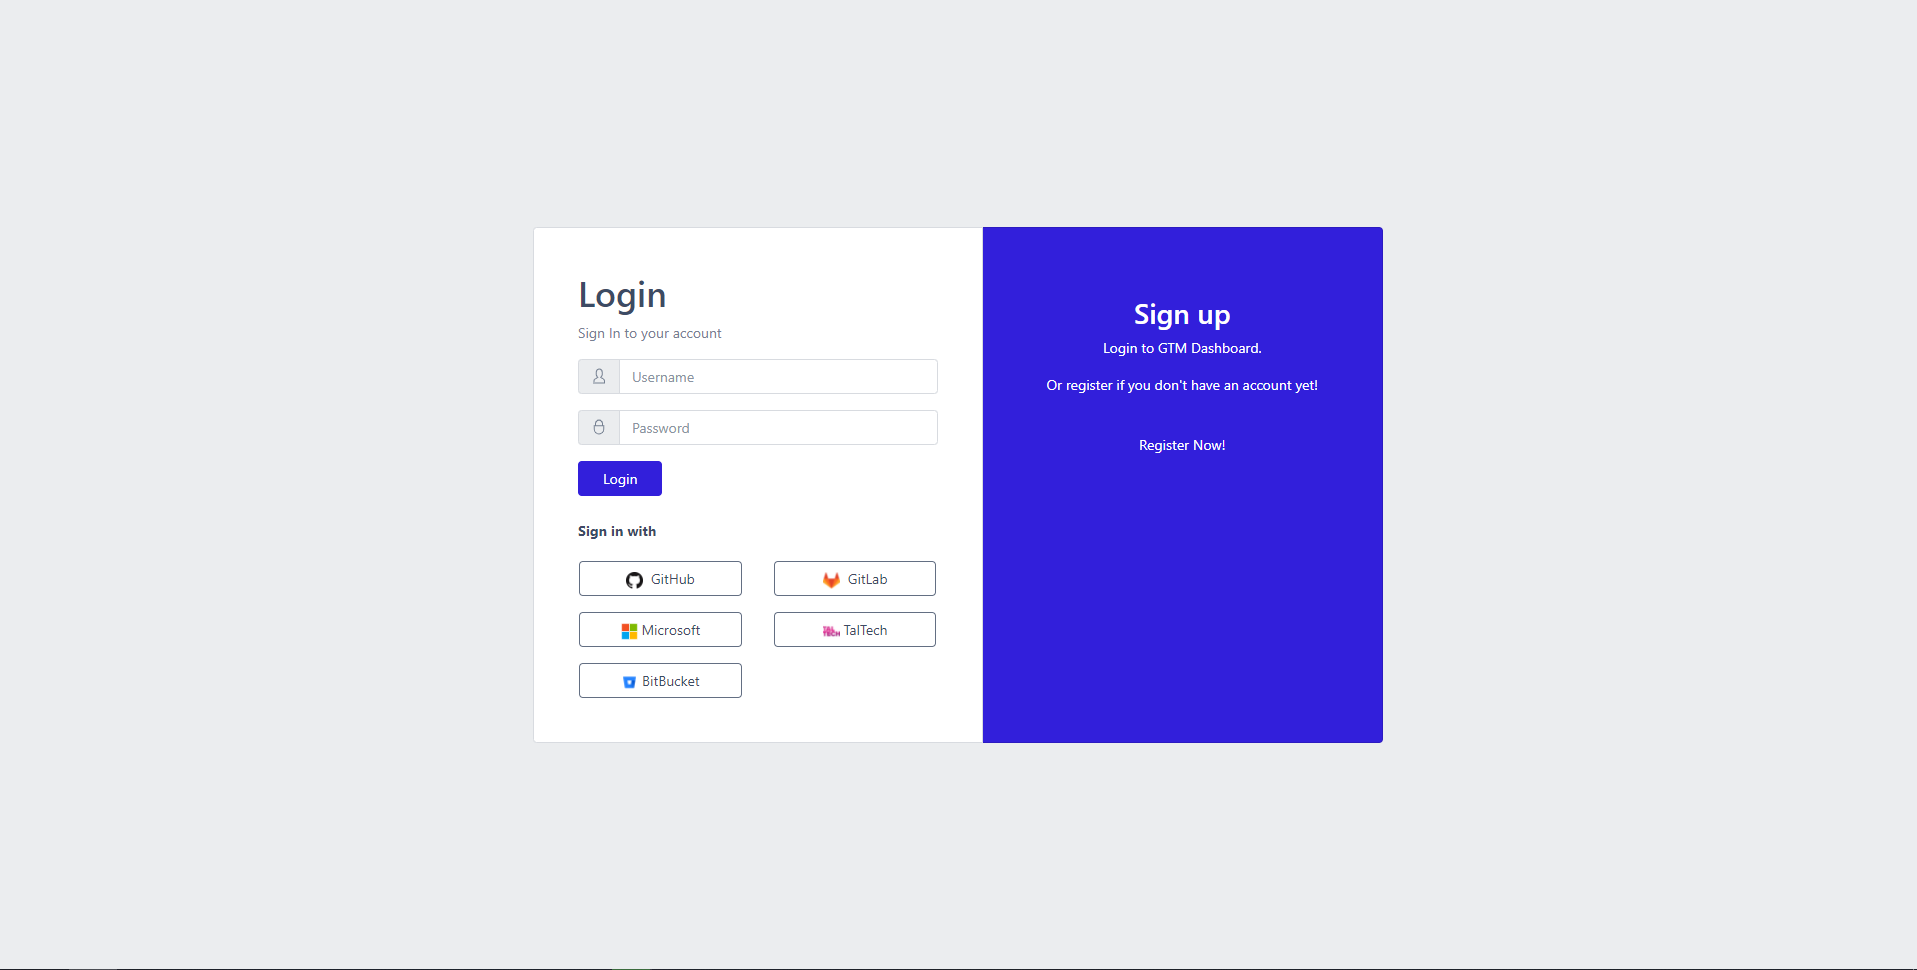
\includegraphics[width=1\textwidth]{figures/views/login}
    \caption{\textit{Login view.}}
    \label{fig:login}
\end{figure}

\begin{figure}[ht]
    \centering
    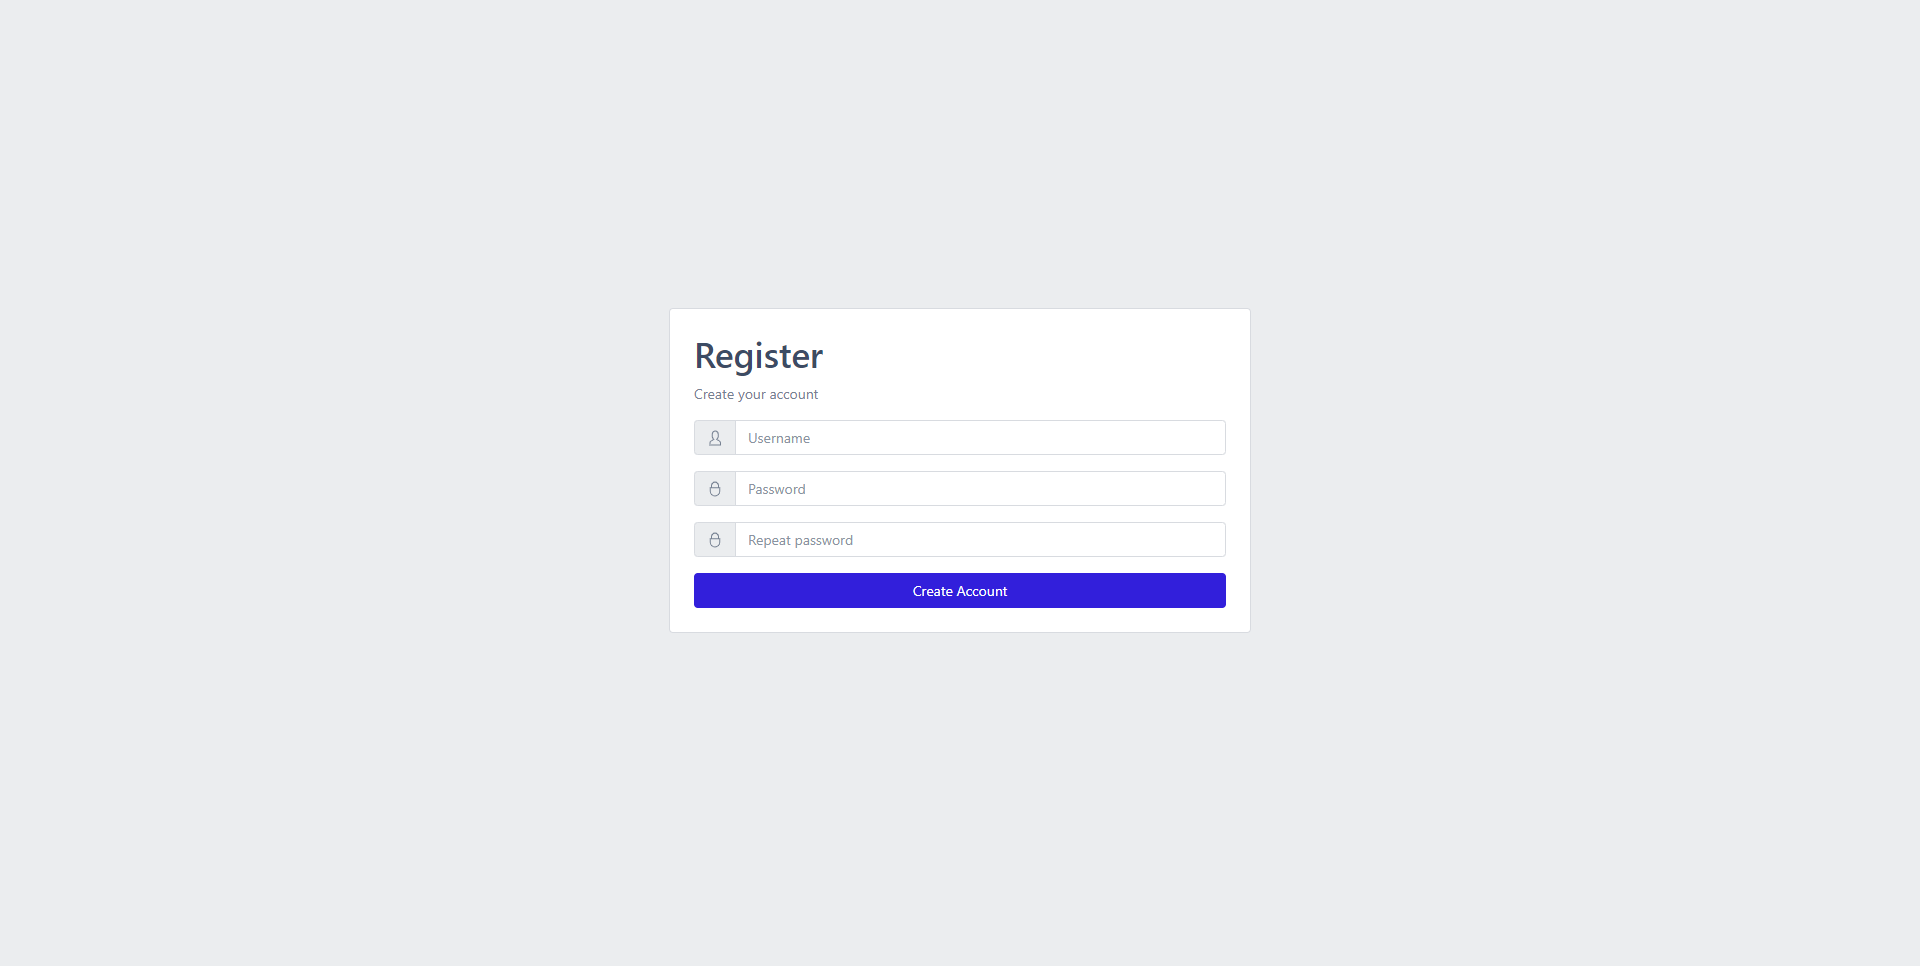
\includegraphics[width=1\textwidth]{figures/views/register}
    \caption{\textit{Register view.}}
    \label{fig:register}
\end{figure}

\begin{figure}[ht]
    \centering
    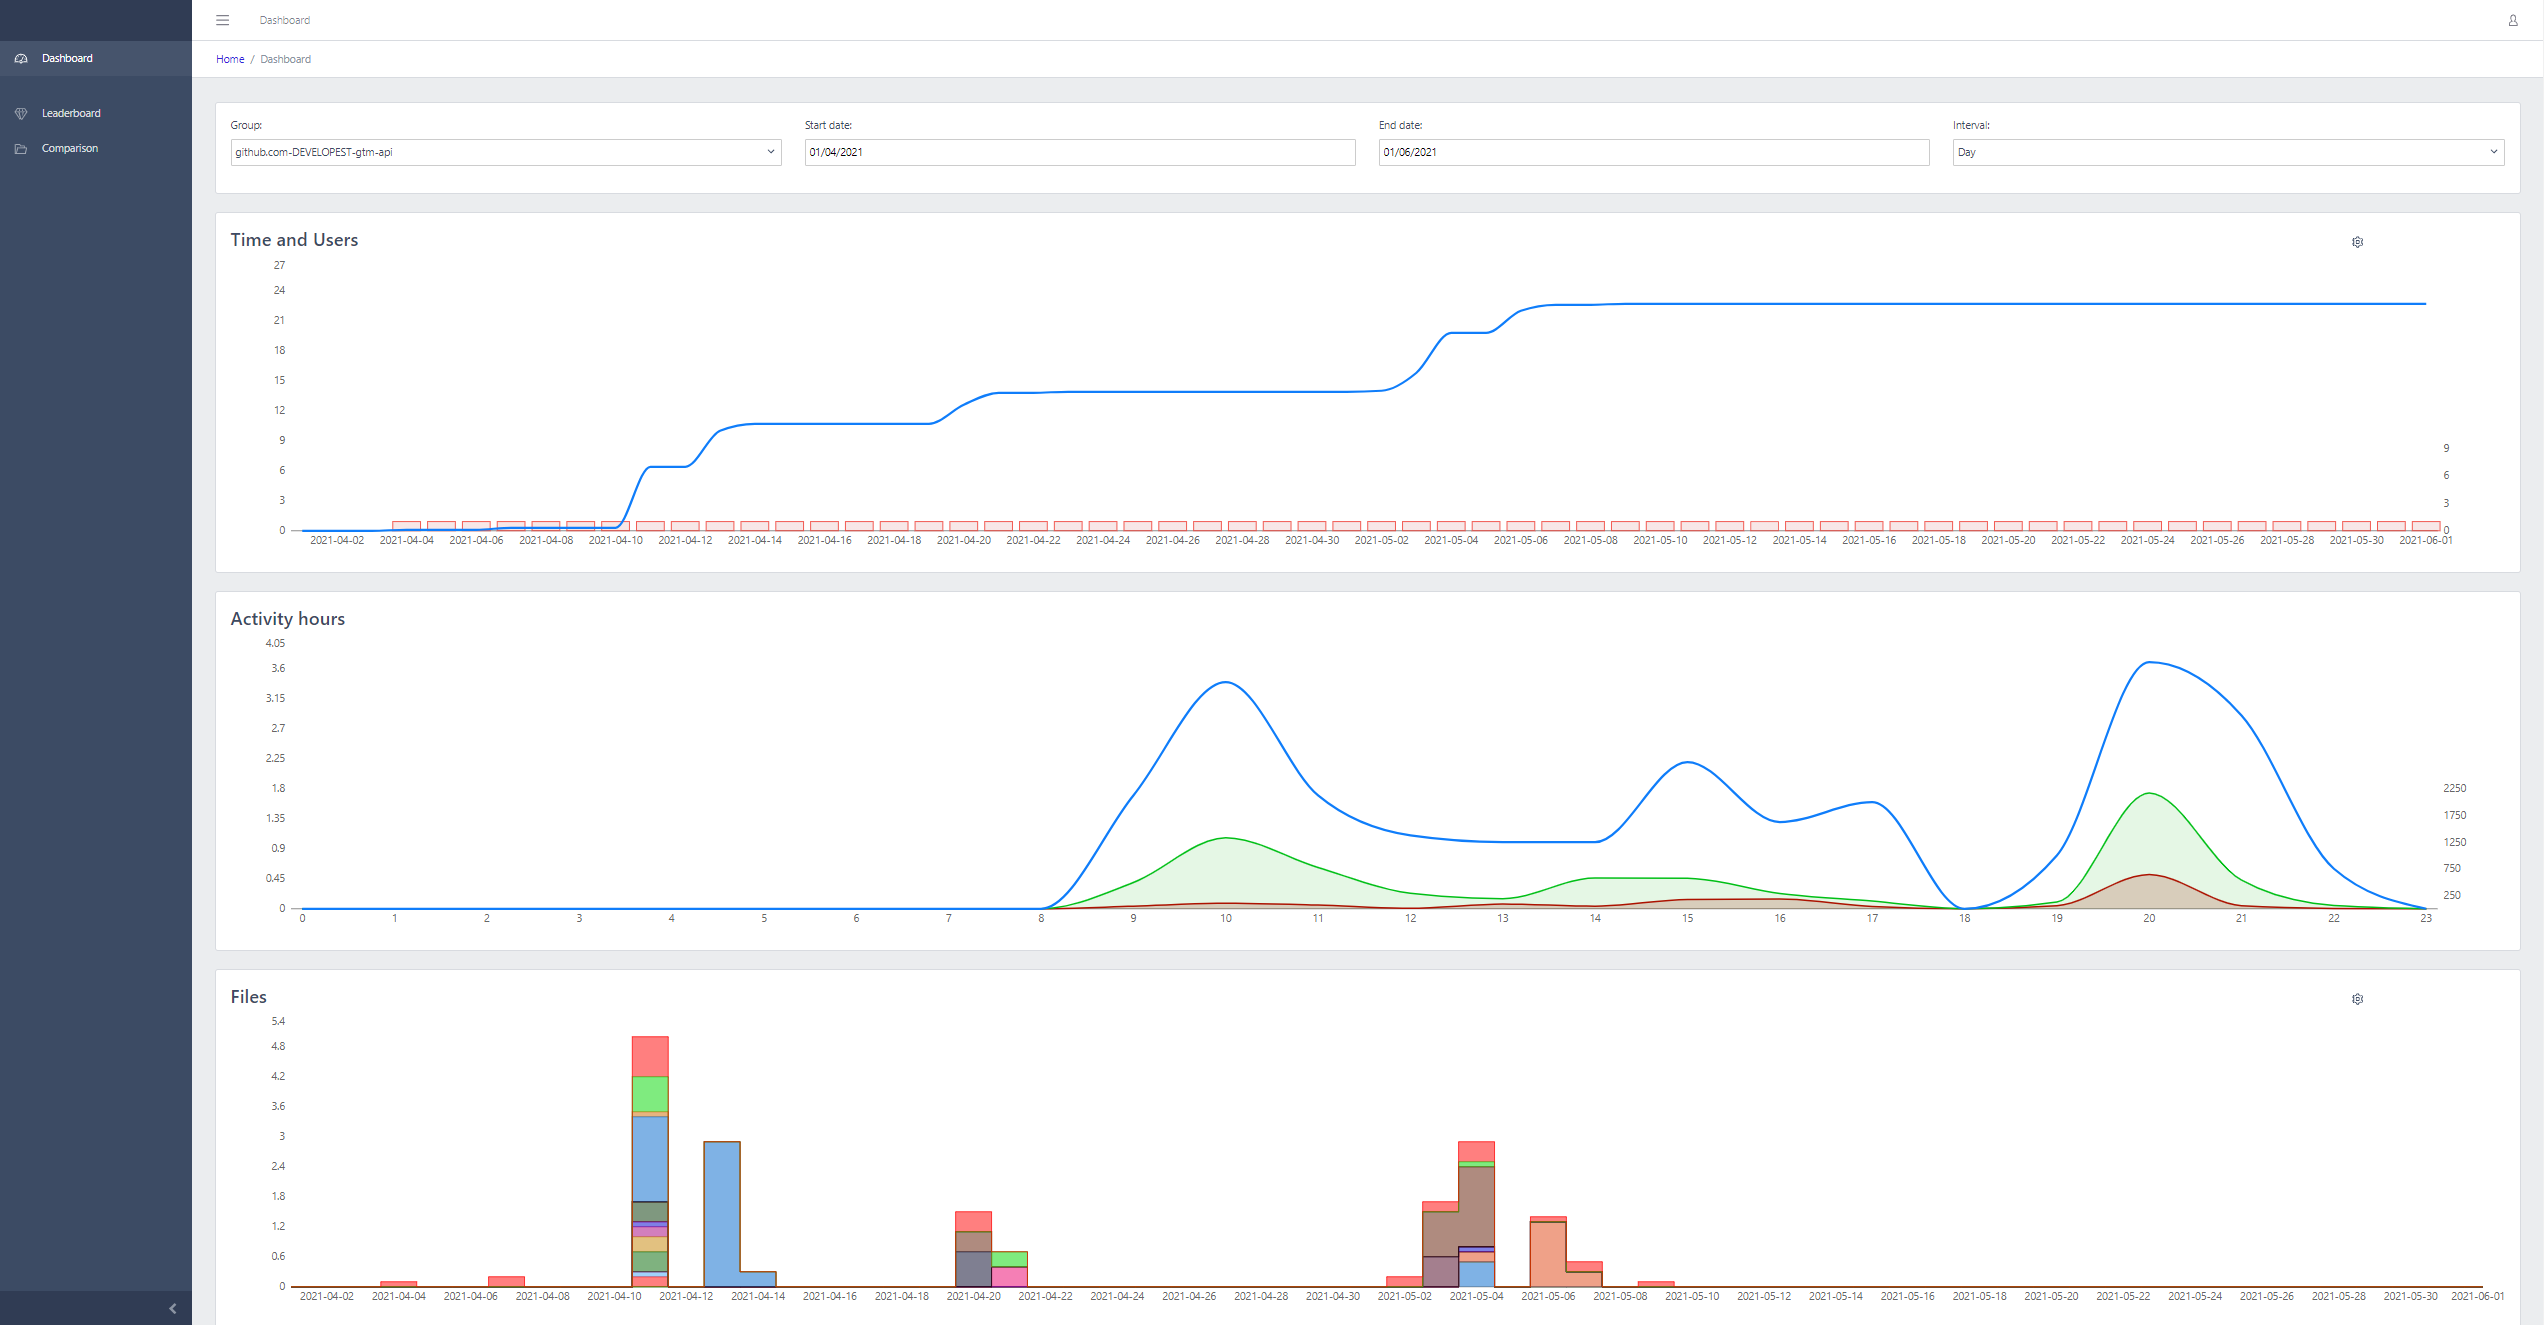
\includegraphics[width=1\textwidth]{figures/views/dashboard}
    \caption{\textit{Dashboard view.}}
    \label{fig:dashboard}
\end{figure}

\begin{figure}[ht]
    \centering
    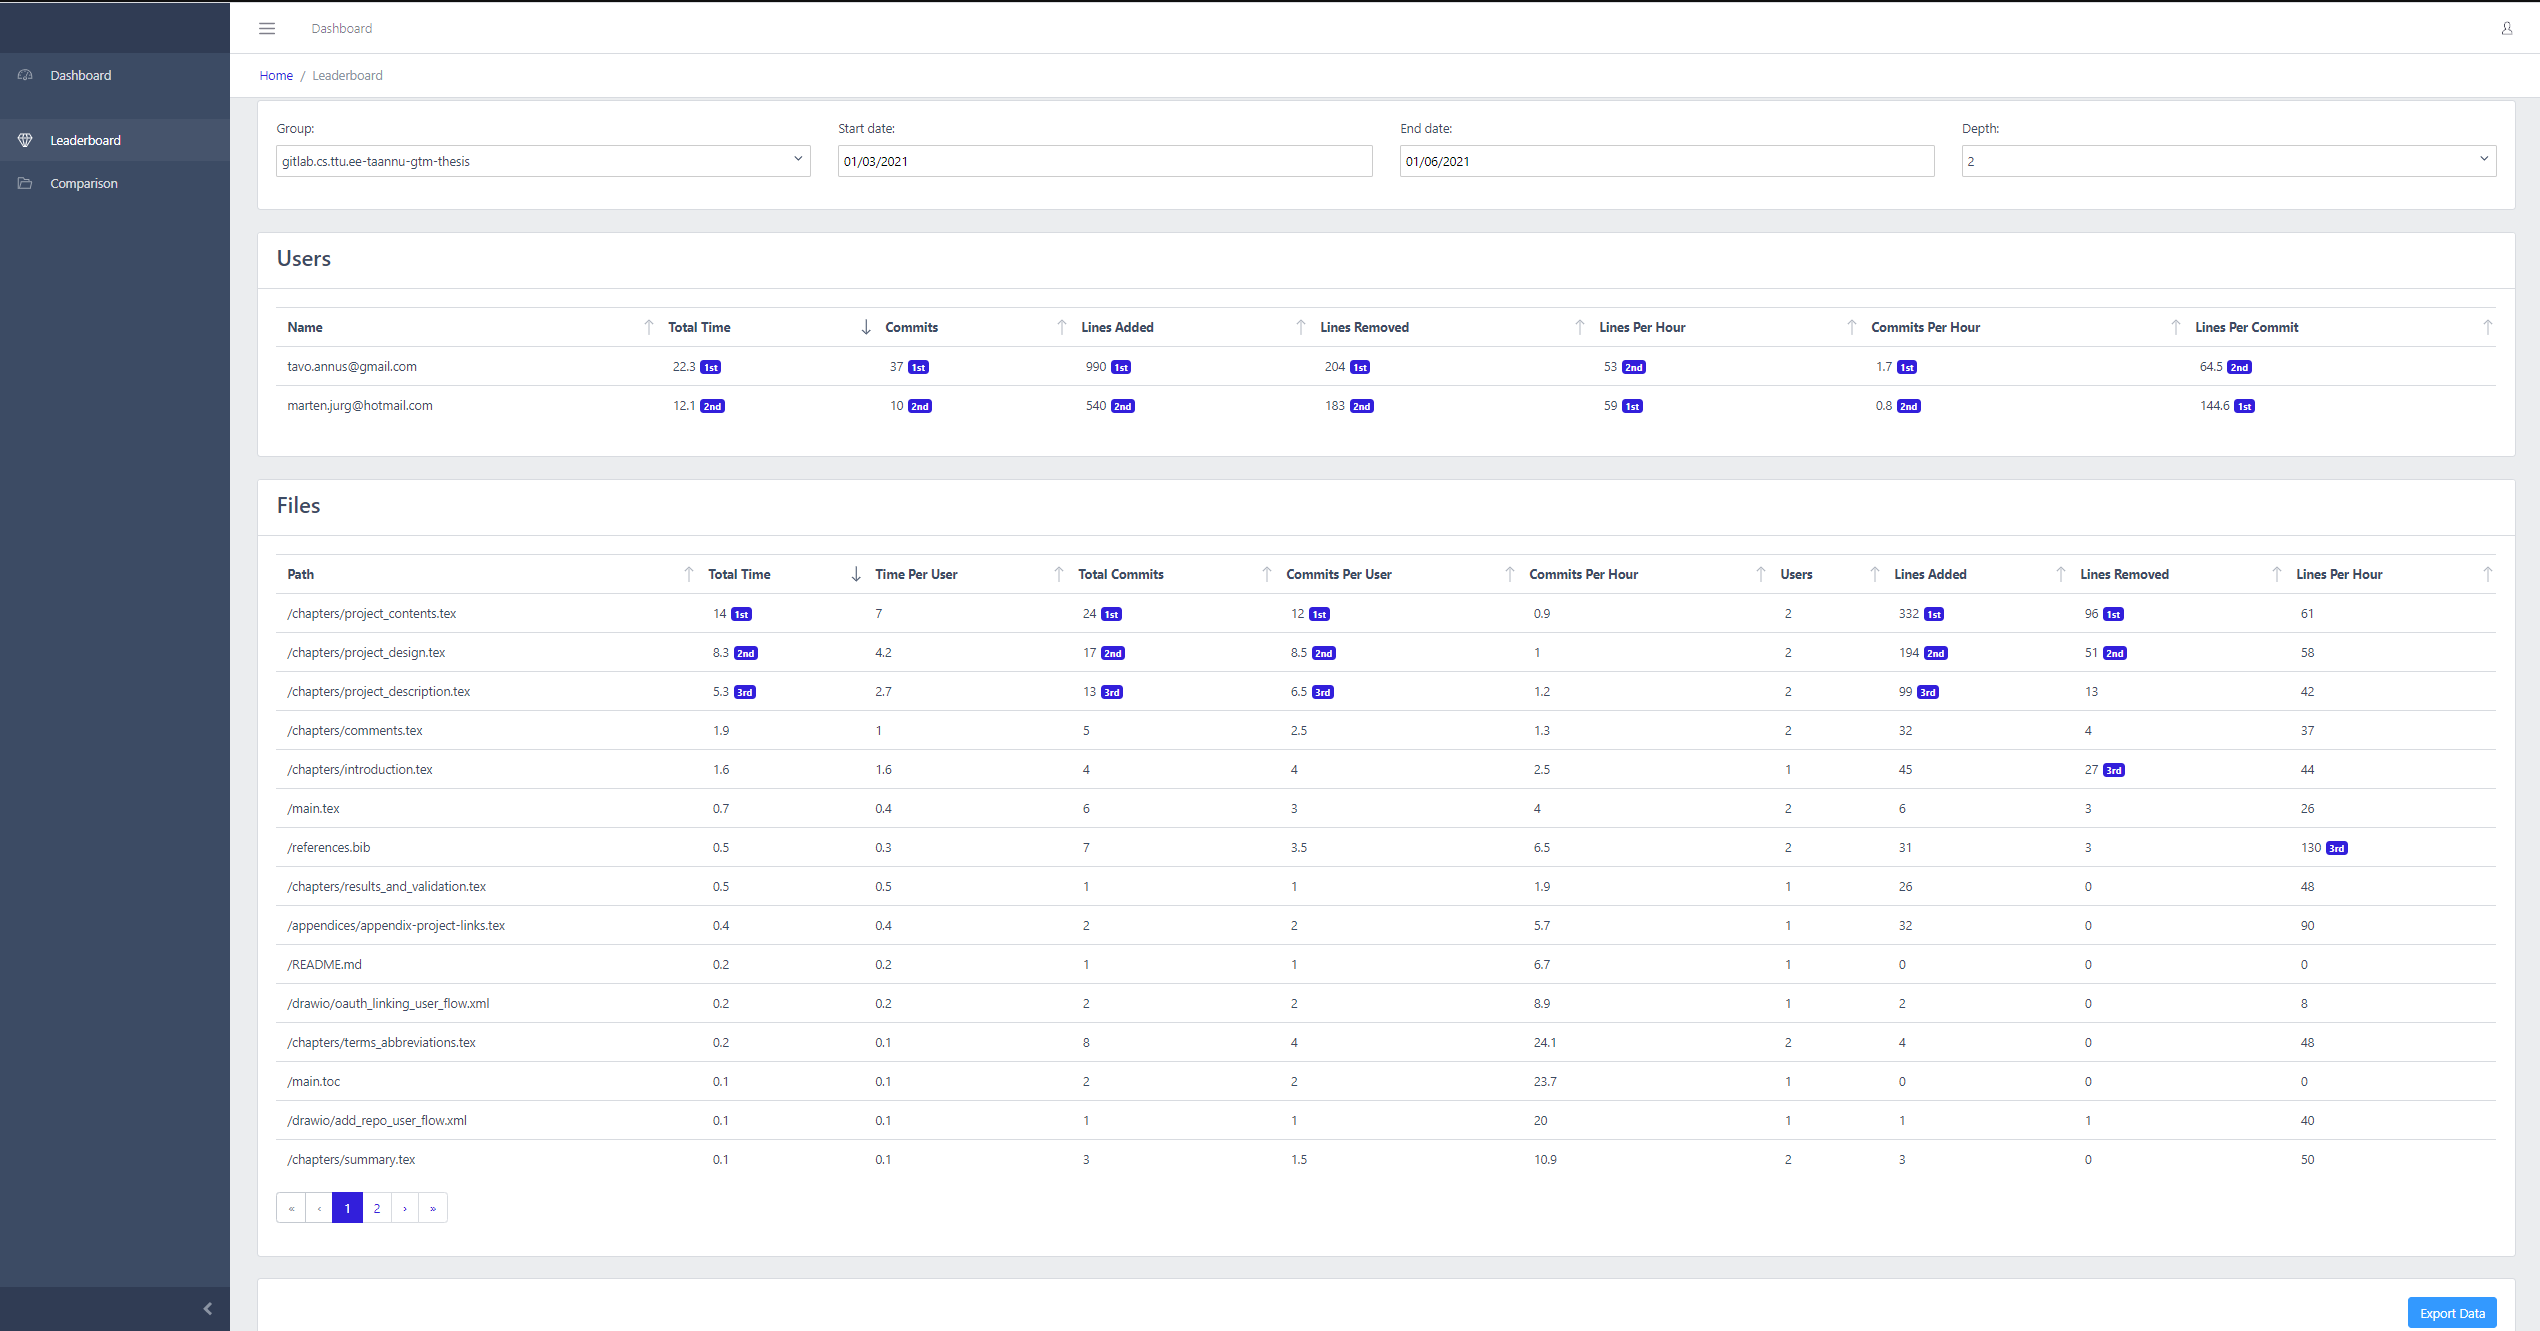
\includegraphics[width=1\textwidth]{figures/views/leaderboard}
    \caption{\textit{Leaderboard view.}}
    \label{fig:leaderboard}
\end{figure}

\begin{figure}[ht]
    \centering
    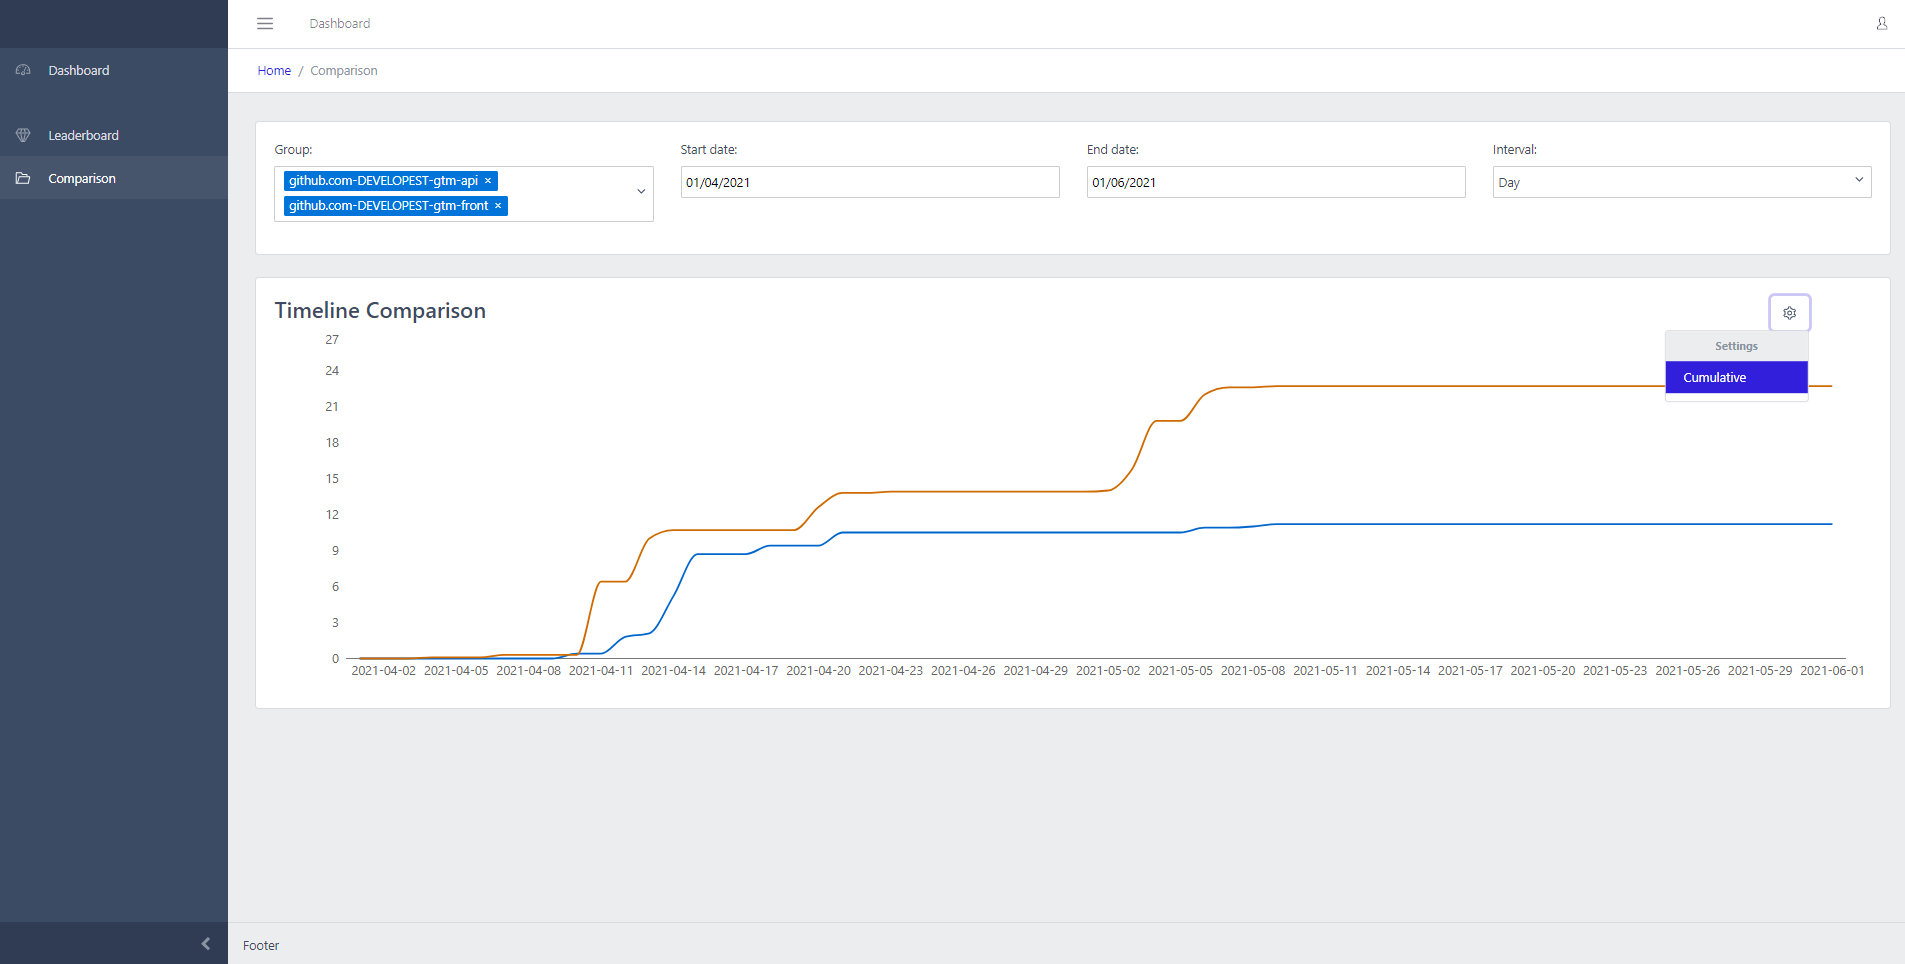
\includegraphics[width=1\textwidth]{figures/views/comparison}
    \caption{\textit{Comparison view.}}
    \label{fig:comparison}
\end{figure}

\begin{figure}[ht]
    \centering
    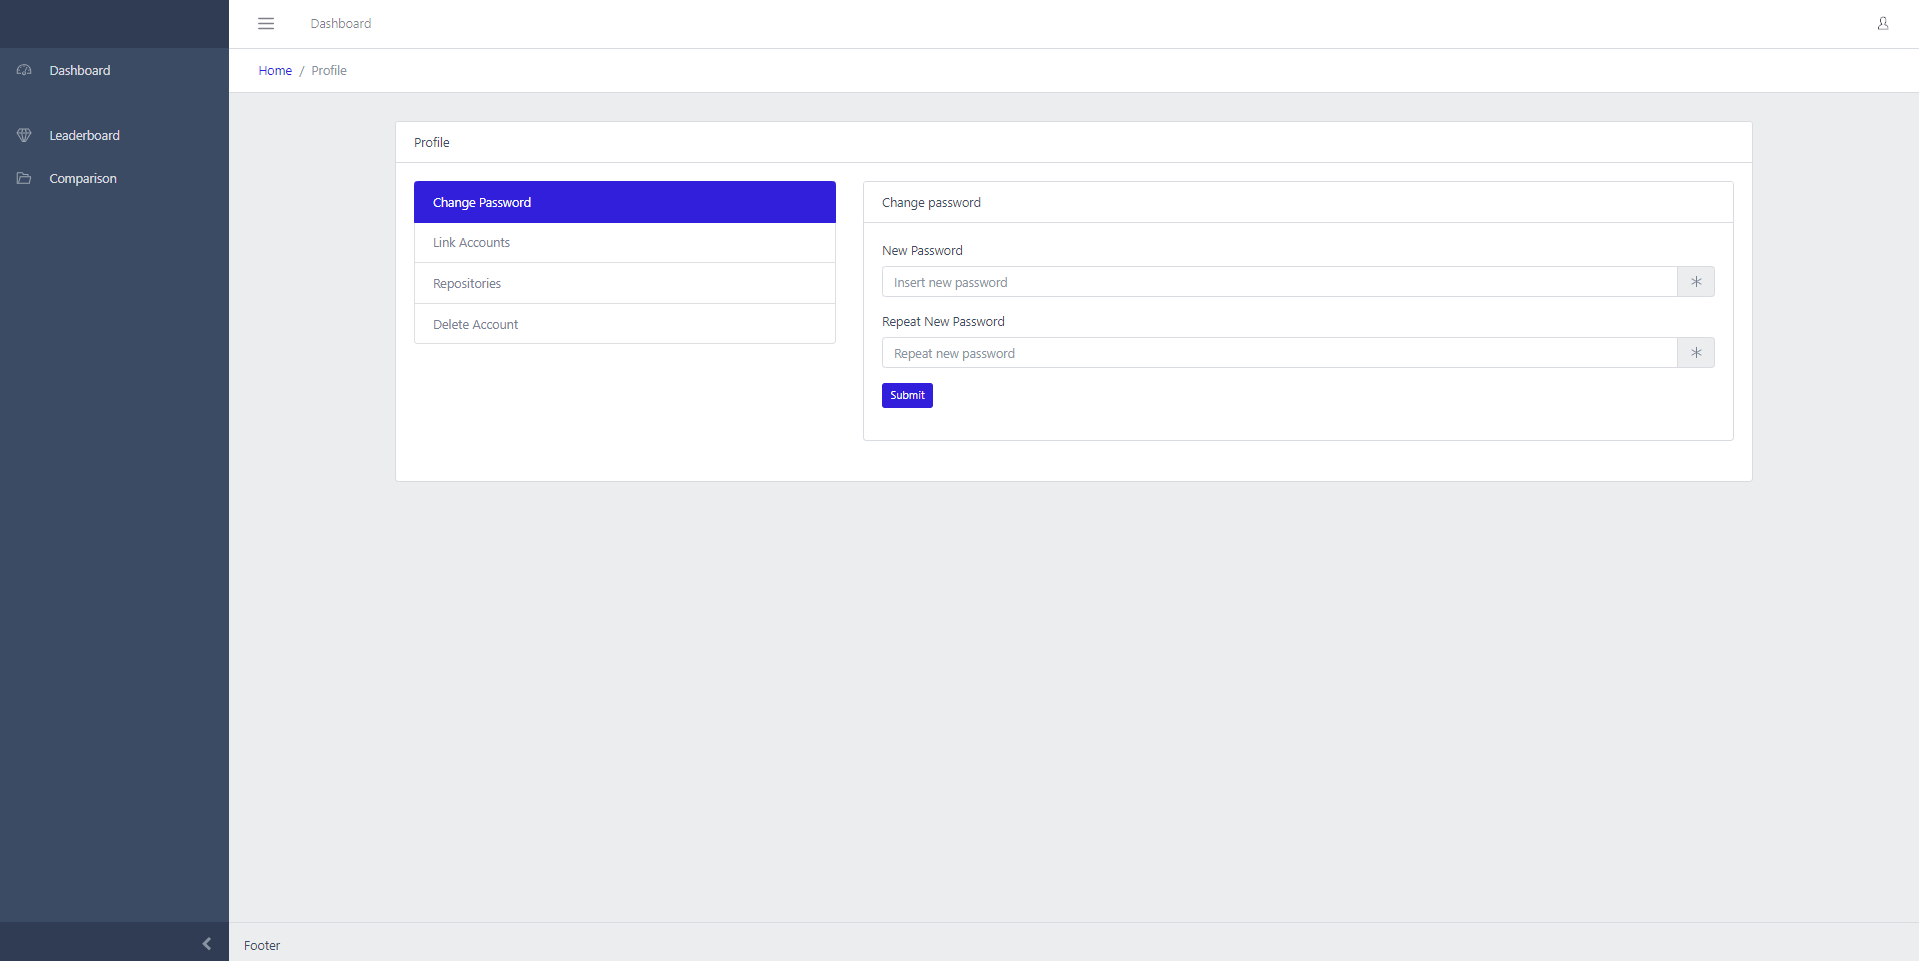
\includegraphics[width=1\textwidth]{figures/views/change_password}
    \caption{\textit{Change password view.}}
    \label{fig:change_password}
\end{figure}

\begin{figure}[ht]
    \centering
    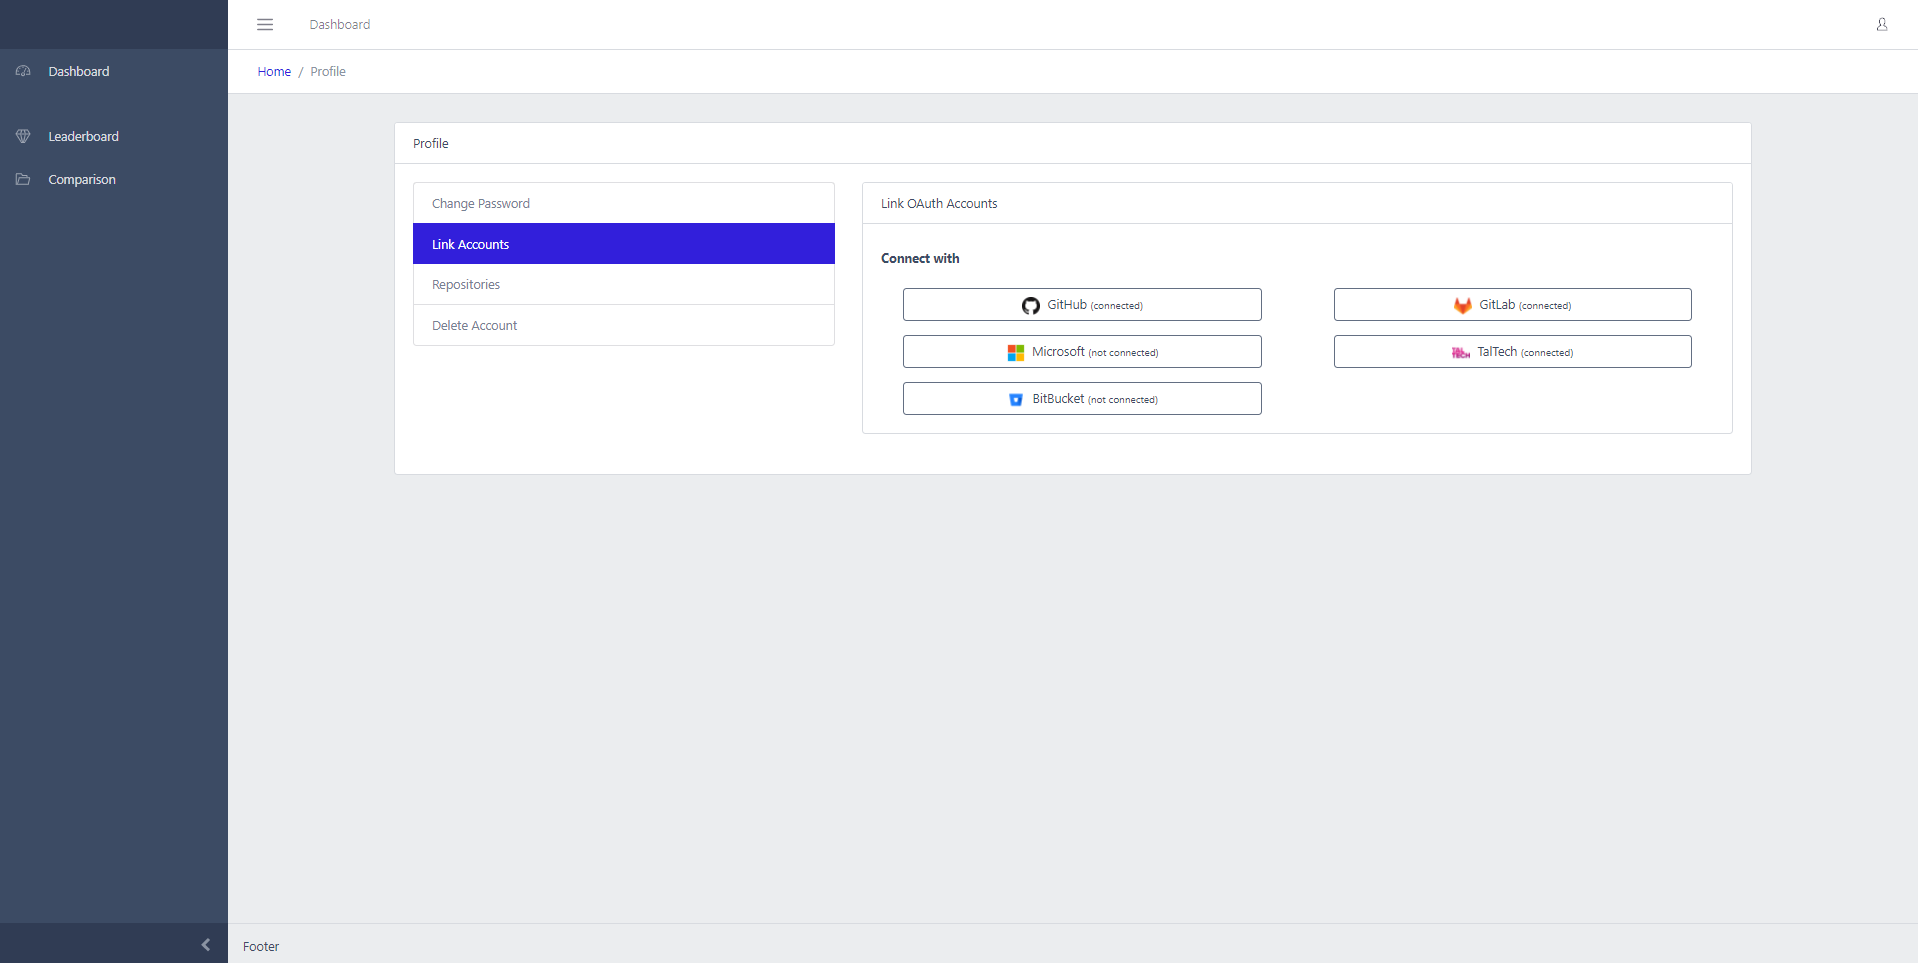
\includegraphics[width=1\textwidth]{figures/views/link_accounts}
    \caption{\textit{Link accounts view.}}
    \label{fig:link_accounts}
\end{figure}

\begin{figure}[ht]
    \centering
    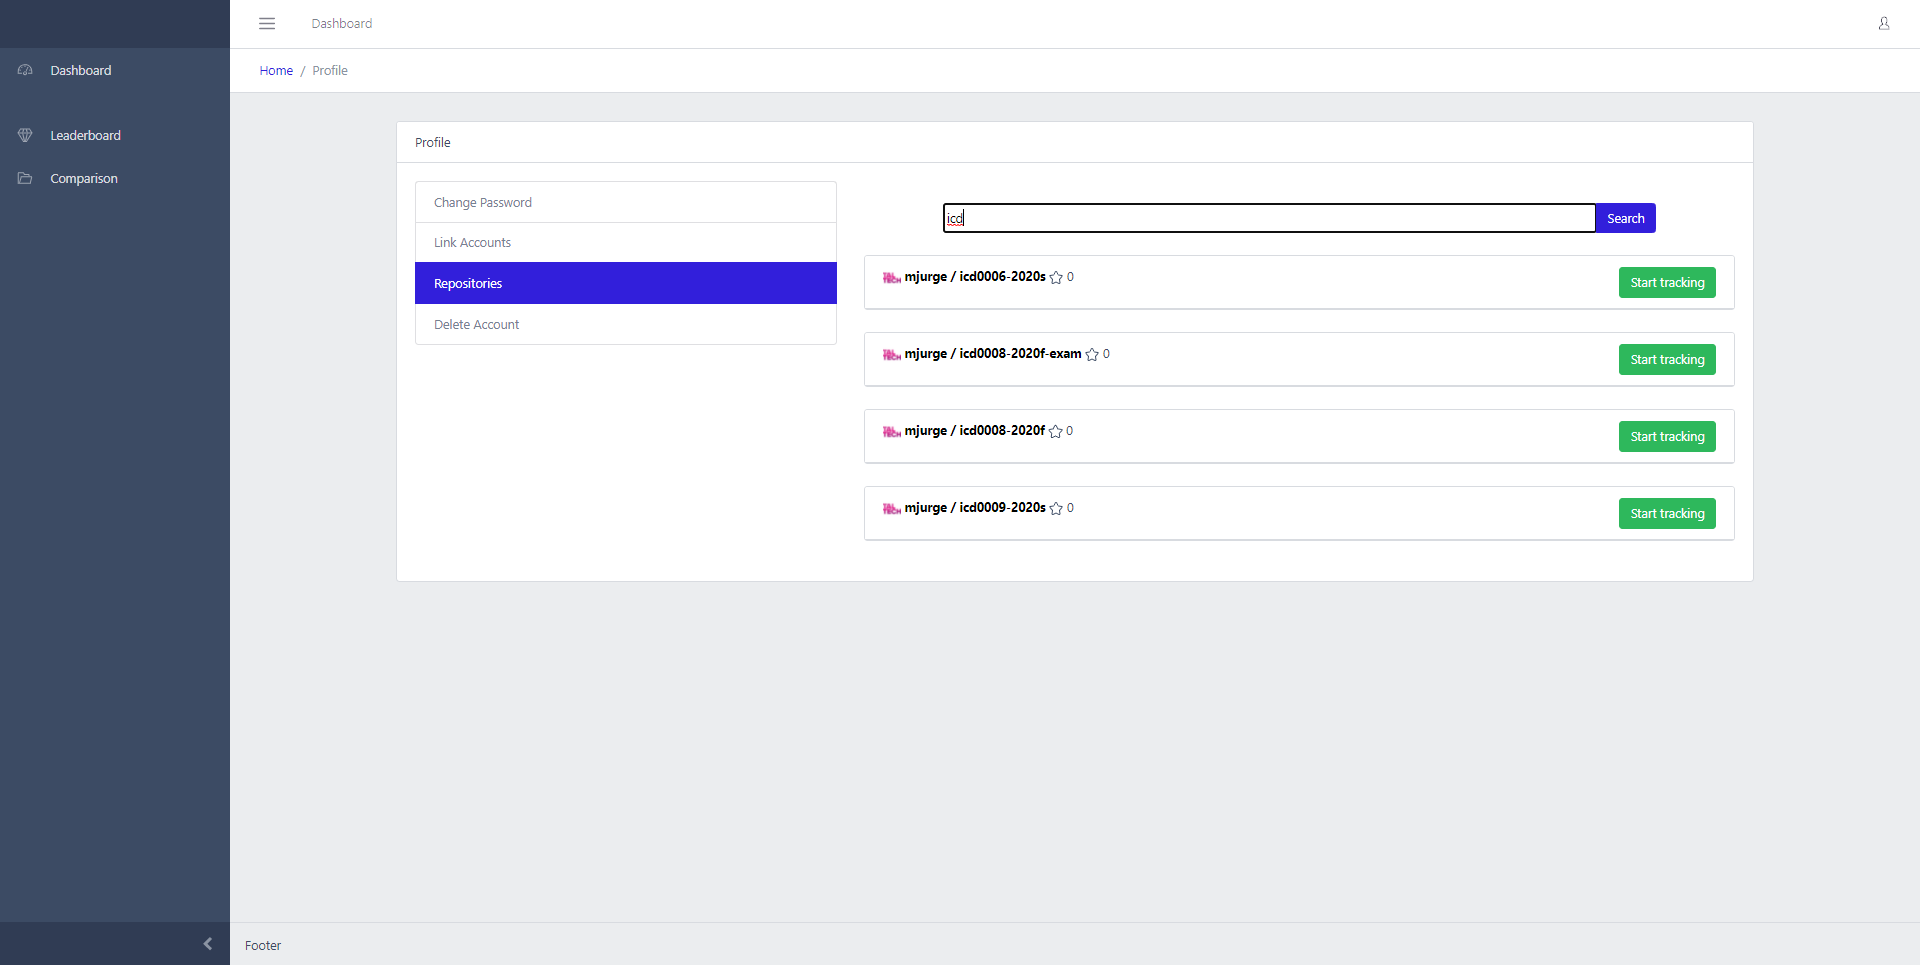
\includegraphics[width=1\textwidth]{figures/views/repositories}
    \caption{\textit{Repositories view.}}
    \label{fig:repositories}
\end{figure}

\begin{figure}[ht]
    \centering
    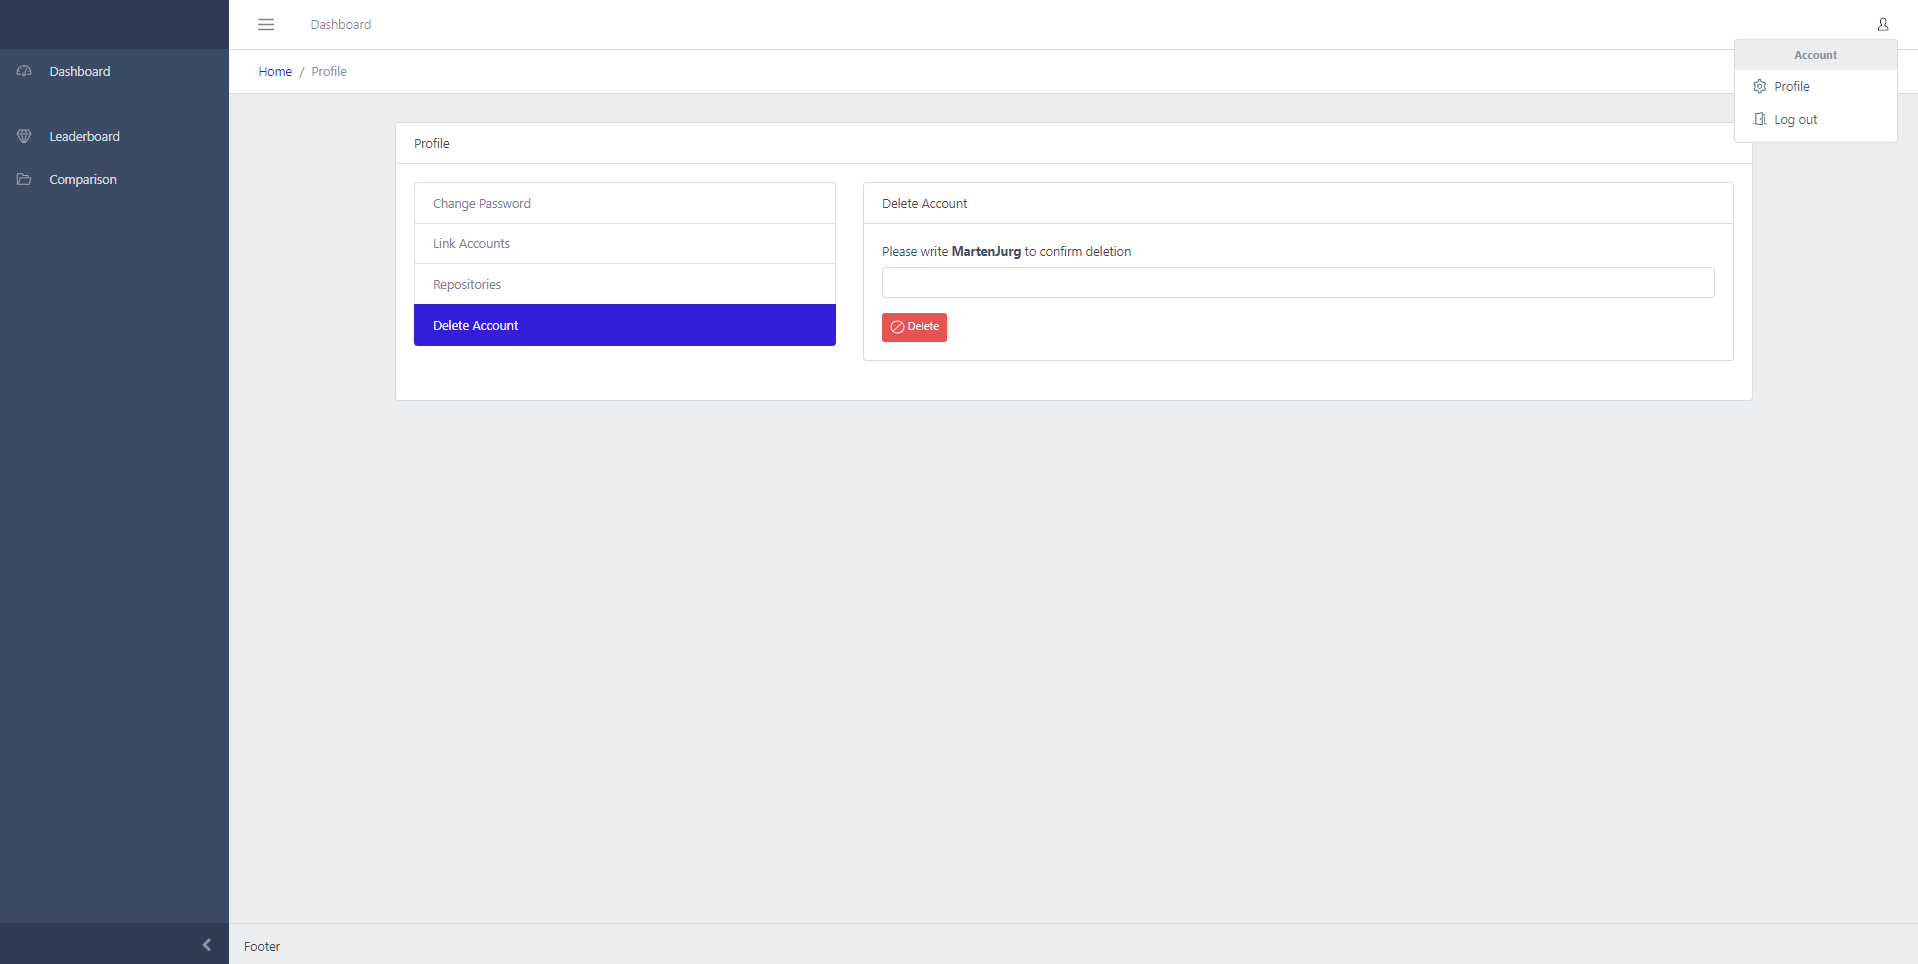
\includegraphics[width=1\textwidth]{figures/views/delete_account}
    \caption{\textit{Delete account view.}}
    \label{fig:delete_account}
\end{figure}


\end{document}
